\documentclass[twocolumn]{aa}

% to make colores in title page
\usepackage{tikz}
\usetikzlibrary{trees}
% to write code with appropriate fonts
\usepackage{listings}
\usepackage{graphicx}
\usepackage{amsmath,amsfonts,amssymb}
\usepackage{txfonts}
\usepackage{color}
\usepackage{textcomp}
%\usepackage{fixltx2e}
\usepackage{natbib}
\usepackage{import}
%\usepackage{caption,subcaption}
%\usepackage{epsfig}
\usepackage{float}
%\usepackage{stfloats}
\usepackage{dblfloatfix}
\usepackage{afterpage}
\usepackage{ifthen}
\usepackage[morefloats=12]{morefloats}
\usepackage{placeins}
\usepackage{multicol}
%\usepackage[breaklinks,colorlinks,citecolor=blue]{hyperref}
\bibpunct{(}{)}{;}{a}{}{,}
\usepackage[switch]{lineno}
\definecolor{linkcolor}{rgb}{0.6,0,0}
\definecolor{citecolor}{rgb}{0,0,0.75}
\definecolor{urlcolor}{rgb}{0.12,0.46,0.7}
\usepackage[breaklinks, colorlinks, urlcolor=urlcolor,
    linkcolor=linkcolor,citecolor=citecolor,pdfencoding=auto]{hyperref}
\hypersetup{linktocpage}
\usepackage{bold-extra}

%Planck style file, to be used with A&A style to produce Planck papers for publication.
%
% version 28 September 2010 --- useful macros --- CRL
% version 17 October 2010   --- first cut at important instrument values, from Daniele Mennella and
%                               Francois Bouchet, 13 October 2010 --- CRL
% version 18 October 2010   --- LFI FWHM changed to one value per feed, rather than M & S separately
%                               LFI FWHM uncertainties added for individual feeds.  Corrections made
%                               to LFI values. --- Andrea Zacchei
% version 24 October 2010   --- added to and corrected definitions.  No changes made to instrument
%                               quantities. --- CRL 
% version 31 October 2010   --- added definition of \muKHz. --- CRL
%
% version 15 November 2010  --- fixed conflict with aa.cls in definition of \endtable
%                               by naming the command below "\endPlancktable".  See section
%                               13.16 of the Style Guide.
%
% version 06 December 2010  --- Set up names with and without units.
%                               Add \allearlypapers command to ensure that all early papers are
%                               included in the reference list.
%                               Define macro for the name of the 4He JT cooler.
%
% version 07 December 2010  --- removed extraneous "planck2011-1.2" entry in \allearlypapers
%
% version 12 December 2010  --- added \endPlancktablewide command to set tablenotes to the full
%                               page width in the \begin{table*}...\end{table*} environment when
%                               the ``twocolumn'' option is specified in the \documentclass command.
%                               (It would be more elegant to extract the appropriate width from the
%                               aa.cls system at the time of execution, but that is buried more
%                               deeply in the system than I investigated.)
%
% version 05 January 2011   --- added unit \MJysr.  HFI performance values updated per FRB email
%                               01/05/2011 02:38-0800, and Brendan Crill email 01/05/2011 18:08 -0800.
%
% version 06 January 2011   --- changed \scriptscriptstyle primes to \scriptstyle, to better match the
%                               tx fonts used by A&A.
%
% version 07 January 2011   --- modified \allearlypapers to correspond with final early paper list.  
%                               Fixed 545 GHz center frequency.
%
% version 07 January 2011b  --- changed LFI white-noise sensitivity numbers to correct problem with units
%
% version 05 July 2011      --- added \Msol and \Lsol to get the symbols for solar mass and luminosity.
%                               Deleted previous definitions of \solar and \sol, which were equivalent
%                               to the new \Msol.
%
% version 16 August 2011    --- changed comments on \endPlancktable and \endPlancktablewide for clarity
%
% version 11 September 2011 --- changed definition of \tablenote to make footnote labels italic, as per A\&A
%
% version 26 April 2011     --- changed definition of \Planck to agree with what is said in the Style Guide (!)
%
% version 04 Dec 2013       --- included 2013 results references
%
% version 17 Jan 2014       --- included fix to bibtex file v4.3, i.e. \providecommand{\sorthelp}[1]{}
%
% version 26 Jul 2014       --- fixed incompatibility problem with aa.cls v8.0 and v8.2.  v8.2 should now be used
%                               for all Planck papers.
%                           --- fixed problem in definition of "\all2013resultspapers" that introduced a blanck
%                               into the reference to p06b.
%                           --- removed all the parameter definition stuff at the end.  We weren't using it, and
%                               it took up a lot of space.
%
% version 28 Jan 2015       --- added "\alltwentyfiftennresultspapers" and corrected "\all2013resultspapers" to
%                               "\all20thirteenresultspapers",
%
% Usage:  after the \documentclass[traditabstract]{aa} command in the La\TeX\ input file,
%         add this command:      \input Planck.tex


\def\setsymbol#1#2{\expandafter\def\csname #1\endcsname{#2}}
\def\getsymbol#1{\csname #1\endcsname}

%-----------------------------------------------------------------------
% Planck
%-----------------------------------------------------------------------
\def\Planck{\textit{Planck}}

%-----------------------------------------------------------------------
% The Planck Helium-4 JT cooler
%-----------------------------------------------------------------------
\def\HeJT{$^4$He-JT}

%-----------------------------------------------------------------------
% To include all Planck Early Results papers in the reference lists
%-----------------------------------------------------------------------
\def\allearlypapers{\nocite{planck2011-1.1, planck2011-1.3, planck2011-1.4, planck2011-1.5, planck2011-1.6, planck2011-1.7, planck2011-1.10, planck2011-1.10sup, planck2011-5.1a, planck2011-5.1b, planck2011-5.2a, planck2011-5.2b, planck2011-5.2c, planck2011-6.1, planck2011-6.2, planck2011-6.3a, planck2011-6.4a, planck2011-6.4b, planck2011-6.6, planck2011-7.0, planck2011-7.2, planck2011-7.3, planck2011-7.7a, planck2011-7.7b, planck2011-7.12, planck2011-7.13}}

%-----------------------------------------------------------------------
% To include all Planck 2013 Results papers in the reference lists
%-----------------------------------------------------------------------
\def\alltwentythirteenresultspapers{\nocite{planck2013-p01, planck2013-p02, planck2013-p02a, planck2013-p02d, planck2013-p02b, planck2013-p03, planck2013-p03c, planck2013-p03f, planck2013-p03d, planck2013-p03e, planck2013-p01a, planck2013-p06, planck2013-p03a, planck2013-pip88, planck2013-p08, planck2013-p11, planck2013-p12, planck2013-p13, planck2013-p14, planck2013-p15, planck2013-p05b, planck2013-p17, planck2013-p09, planck2013-p09a, planck2013-p20, planck2013-p19, planck2013-pipaberration, planck2013-p05, planck2013-p05a, planck2013-pip56, planck2013-p06b, planck2013-p01a}}

%-----------------------------------------------------------------------
% To include all Planck 2015 Results papers in the reference lists
%-----------------------------------------------------------------------
\def\alltwentyfifteenresultspapers{\nocite{planck2014-a01, planck2014-a03, planck2014-a04, planck2014-a05, planck2014-a06, planck2014-a07, planck2014-a08, planck2014-a09, planck2014-a11, planck2014-a12, planck2014-a13, planck2014-a14, planck2014-a15, planck2014-a16, planck2014-a17, planck2014-a18, planck2014-a19, planck2014-a20, planck2014-a22, planck2014-a24, planck2014-a26, planck2014-a28, planck2014-a29, planck2014-a30, planck2014-a31, planck2014-a35, planck2014-a36, planck2014-a37, planck2014-ES}}

%-----------------------------------------------------------------------
% Tables
%-----------------------------------------------------------------------
\newbox\tablebox    \newdimen\tablewidth
\def\leaderfil{\leaders\hbox to 5pt{\hss.\hss}\hfil}
%
% use the following definition of \endPlancktable for ApJ style notes to tables, set to the 
%         width of the table
% \def\endPlancktable{\tablewidth=\wd\tablebox 
%
% use the following definitions of \endPlancktable and \endPlancktablewide for A&A style notes 
% set to one-column  or full-page width, respectively
\def\endPlancktable{\tablewidth=\columnwidth 
    $$\hss\copy\tablebox\hss$$
    \vskip-\lastskip\vskip -2pt}
\def\endPlancktablewide{\tablewidth=\textwidth 
    $$\hss\copy\tablebox\hss$$
    \vskip-\lastskip\vskip -2pt}
\def\tablenote#1 #2\par{\begingroup \parindent=0.8em
    \abovedisplayshortskip=0pt\belowdisplayshortskip=0pt
    \noindent
    $$\hss\vbox{\hsize\tablewidth \hangindent=\parindent \hangafter=1 \noindent
    \hbox to \parindent{$^#1$\hss}\strut#2\strut\par}\hss$$
    \endgroup}
\def\doubleline{\vskip 3pt\hrule \vskip 1.5pt \hrule \vskip 5pt}

%-----------------------------------------------------------------------
% useful macros
%-----------------------------------------------------------------------
%
\def\L2{\ifmmode L_2\else $L_2$\fi}
%
\def\dtt{\Delta T/T}
\def\DeltaT{\ifmmode \Delta T\else $\Delta T$\fi}
\def\deltat{\ifmmode \Delta t\else $\Delta t$\fi}
\def\fknee{\ifmmode f_{\rm knee}\else $f_{\rm knee}$\fi}
\def\Fmax{\ifmmode F_{\rm max}\else $F_{\rm max}$\fi}
%
\def\solar{\ifmmode{\rm M}_{\mathord\odot}\else${\rm M}_{\mathord\odot}$\fi}
\def\Msolar{\ifmmode{\rm M}_{\mathord\odot}\else${\rm M}_{\mathord\odot}$\fi}
\def\Lsolar{\ifmmode{\rm L}_{\mathord\odot}\else${\rm L}_{\mathord\odot}$\fi}
%
\def\inv{\ifmmode^{-1}\else$^{-1}$\fi}
\def\mo{\ifmmode^{-1}\else$^{-1}$\fi}
\def\sup#1{\ifmmode ^{\rm #1}\else $^{\rm #1}$\fi}
\def\expo#1{\ifmmode \times 10^{#1}\else $\times 10^{#1}$\fi}
%
\def\,{\thinspace}
\def\lsim{\mathrel{\raise .4ex\hbox{\rlap{$<$}\lower 1.2ex\hbox{$\sim$}}}}
\def\gsim{\mathrel{\raise .4ex\hbox{\rlap{$>$}\lower 1.2ex\hbox{$\sim$}}}}
\let\lea=\lsim
\let\gea=\gsim
\def\simprop{\mathrel{\raise .4ex\hbox{\rlap{$\propto$}\lower 1.2ex\hbox{$\sim$}}}}
%
\def\deg{\ifmmode^\circ\else$^\circ$\fi}
\def\pdeg{\ifmmode $\setbox0=\hbox{$^{\circ}$}\rlap{\hskip.11\wd0 .}$^{\circ}
          \else \setbox0=\hbox{$^{\circ}$}\rlap{\hskip.11\wd0 .}$^{\circ}$\fi}
\def\arcs{\ifmmode {^{\scriptstyle\prime\prime}}
          \else $^{\scriptstyle\prime\prime}$\fi}
\def\arcm{\ifmmode {^{\scriptstyle\prime}}
          \else $^{\scriptstyle\prime}$\fi}
\newdimen\sa  \newdimen\sb
\def\parcs{\sa=.07em \sb=.03em
     \ifmmode \hbox{\rlap{.}}^{\scriptstyle\prime\kern -\sb\prime}\hbox{\kern -\sa}
     \else \rlap{.}$^{\scriptstyle\prime\kern -\sb\prime}$\kern -\sa\fi}
\def\parcm{\sa=.08em \sb=.03em
     \ifmmode \hbox{\rlap{.}\kern\sa}^{\scriptstyle\prime}\hbox{\kern-\sb}
     \else \rlap{.}\kern\sa$^{\scriptstyle\prime}$\kern-\sb\fi}
%
\def\ra[#1 #2 #3.#4]{#1\sup{h}#2\sup{m}#3\sup{s}\llap.#4}
\def\dec[#1 #2 #3.#4]{#1\deg#2\arcm#3\arcs\llap.#4}
\def\deco[#1 #2 #3]{#1\deg#2\arcm#3\arcs}
\def\rra[#1 #2]{#1\sup{h}#2\sup{m}}
%
\def\page{\vfill\eject}
\def\dots{\relax\ifmmode \ldots\else $\ldots$\fi}
%
%-----------------------------------------------------------------------
% units
%-----------------------------------------------------------------------
%
\def\WHzsr{\ifmmode $W\,Hz\mo\,sr\mo$\else W\,Hz\mo\,sr\mo\fi}
\def\mHz{\ifmmode $\,mHz$\else \,mHz\fi}
\def\GHz{\ifmmode $\,GHz$\else \,GHz\fi}
\def\mKs{\ifmmode $\,mK\,s$^{1/2}\else \,mK\,s$^{1/2}$\fi}
\def\muKs{\ifmmode \,\mu$K\,s$^{1/2}\else \,$\mu$K\,s$^{1/2}$\fi}
\def\muKRJs{\ifmmode \,\mu$K$_{\rm RJ}$\,s$^{1/2}\else \,$\mu$K$_{\rm RJ}$\,s$^{1/2}$\fi}
\def\muKHz{\ifmmode \,\mu$K\,Hz$^{-1/2}\else \,$\mu$K\,Hz$^{-1/2}$\fi}
\def\MJysr{\ifmmode \,$MJy\,sr\mo$\else \,MJy\,sr\mo\fi}
\def\MJysrmK{\ifmmode \,$MJy\,sr\mo$\,mK$_{\rm CMB}\mo\else \,MJy\,sr\mo\,mK$_{\rm CMB}\mo$\fi}
\def\microns{\ifmmode \,\mu$m$\else \,$\mu$m\fi}
\def\micron{\microns}
\def\muK{\ifmmode \,\mu$K$\else \,$\mu$\hbox{K}\fi}
\def\microK{\ifmmode \,\mu$K$\else \,$\mu$\hbox{K}\fi}
\def\muW{\ifmmode \,\mu$W$\else \,$\mu$\hbox{W}\fi}
\def\kms{\ifmmode $\,km\,s$^{-1}\else \,km\,s$^{-1}$\fi}
\def\kmsMpc{\ifmmode $\,\kms\,Mpc\mo$\else \,\kms\,Mpc\mo\fi}
%
%
%----------------------------------------------------------------------
% set up machinery to list Planck papers in roman numeral order.
%----------------------------------------------------------------------

\providecommand{\sorthelp}[1]{}

\def\WMAP{\textit{WMAP}}
\def\COBE{\textit{COBE}}
\def\QUIET{\textit{QUIET}}
\def\LCDM{$\Lambda$CDM}
\def\ffp{FFP6}
\def\unionmask{U73}
\def\nside{N_{\mathrm{side}}}

\def\healpix{\texttt{HEALPix}}
\def\commander{\texttt{Commander}}
\def\commanderone{\texttt{Commander1}}
\def\commandertwo{\texttt{Commander2}}
\def\commanderthree{\texttt{Commander3}}
\def\ruler{\texttt{Ruler}}
\def\comrul{\texttt{Commander-Ruler}}
\def\CR{\texttt{C-R}}
\def\nilc{\texttt{NILC}}
\def\gnilc{\texttt{GNILC}}
\def\sevem{\texttt{SEVEM}}
\def\smica{\texttt{SMICA}}
\def\CamSpec{\texttt{CamSpec}}
\def\Plik{\texttt{Plik}}
\def\XFaster{\texttt{XFaster}}

\renewcommand{\d}[0]{\vec{d}}
\renewcommand{\t}[0]{\vec{t}}
\newcommand{\A}[0]{\tens{A}}
%\newcommand{\Y}[0]{\tens{Y}}
\newcommand{\Y}[0]{\tens{Y}}
\newcommand{\y}[0]{\vec{y}}
\newcommand{\n}[0]{\vec{n}}
\newcommand{\x}[0]{\vec{x}}
\newcommand{\red}[0]{\color{red}}
\newcommand{\green}[0]{\color{green}}
\newcommand{\s}[0]{\vec{s}}
\renewcommand{\a}[0]{\vec{a}}
\newcommand{\m}[0]{\vec{m}}
\newcommand{\f}[0]{\vec{f}}
\newcommand{\F}[0]{\tens{F}}
\newcommand{\B}[0]{\tens{B}}
\newcommand{\T}[0]{\tens{T}}
\newcommand{\Cp}[0]{\tens{C}}
\renewcommand{\L}[0]{\tens{L}}
\newcommand{\g}[0]{\vec{g}}
\newcommand{\N}[0]{\tens{N}}
\newcommand{\Z}[0]{\tens{Z}}
\newcommand{\I}[0]{\tens{I}}
\newcommand{\M}[0]{\tens{M}}
\newcommand{\iN}[0]{\tens{N}^{-1}}
\newcommand{\iM}[0]{\tens{M}^{-1}}
\newcommand{\w}[0]{\vec{w}}
\renewcommand{\S}[0]{\tens{S}}
\renewcommand{\r}[0]{\vec{r}}
\renewcommand{\u}[0]{\vec{u}}
\newcommand{\q}[0]{\vec{q}}
\renewcommand{\v}[0]{\vec{v}}
\renewcommand{\P}[0]{\tens{P}}
\newcommand{\R}[0]{\tens{R}}
\newcommand{\dt}[0]{d_t}
\newcommand{\di}[0]{d_i}
\newcommand{\nt}[0]{n_t}
\newcommand{\st}[0]{s_t}
\newcommand{\Dbp}[0]{\Delta_{\mathrm{bp}}}
\newcommand{\mt}[0]{m_t}
\newcommand{\ft}[0]{f_t}
\newcommand{\Te}[0]{T_{\rm e}}
\newcommand{\EM}[0]{\rm EM}
\newcommand{\mathsc}[1]{{\normalfont\textsc{#1}}}
\newcommand{\hi}{\ensuremath{\mathsc {Hi}}}
\newcommand{\bpbold}{\bfseries{\scshape{BeyondPlanck}}}
\newcommand{\BP}{\textsc{BeyondPlanck}}
\newcommand{\cosmoglobe}{\textsc{Cosmoglobe}}
\newcommand{\btoc}{\textsc{bits2cosmology}}
\newcommand{\lfi}[0]{LFI}
\newcommand{\hfi}[0]{HFI}
\newcommand{\npipe}[0]{\texttt{NPIPE}}

\DeclareTextFontCommand{\textbfit}{%
  \fontseries\bfdefault % change series without selecting the font yet
  \itshape
}


\def\bC{\tens{C}}
\def\ba{\vec{a}}
\def\ncha{N_\mathrm{cha}}
\def\nfg{N_\mathrm{fg}}

%\modulolinenumbers[5]
%\linenumbers

\newcommand{\includegraphicsdpi}[3]{
    \pdfimageresolution=#1  % Change the dpi of images
    \includegraphics[#2]{#3}
    \pdfimageresolution=72  % Change it back to the default
}

\renewcommand{\topfraction}{1.0}	% max fraction of floats at top
    \renewcommand{\bottomfraction}{1.0}	% max fraction of floats at bottom
    %   Parameters for TEXT pages (not float pages):
    \setcounter{topnumber}{2}
    \setcounter{bottomnumber}{2}
    \setcounter{totalnumber}{4}     % 2 may work better
    \setcounter{dbltopnumber}{2}    % for 2-column pages
    \renewcommand{\dbltopfraction}{0.9}	% fit big float above 2-col. text
    \renewcommand{\textfraction}{0.04}	% allow minimal text w. figs
    %   Parameters for FLOAT pages (not text pages):
    \renewcommand{\floatpagefraction}{0.9}	% require fuller float pages
	% N.B.: floatpagefraction MUST be less than topfraction !!
    \renewcommand{\dblfloatpagefraction}{0.9}	% require fuller float pages

\def\adj{^{\dagger}}
\def\tp{^{\rm T}}
\def\inv{^{-1}}
\def\lm{{\ell m}}

\begin{document}

\title{\bfseries{From \scshape{BeyondPlanck} to \scshape{Cosmoglobe}:}\\
    Open Science, Reproducibility, and Data Longevity}

%This author list corresponds to \title{Author list for L04\_CMB\_Foregrounds\_Extraction}
%Prepared by M. Lopez-Caniego (Marcos.Lopez.Caniego@sciops.esa.int), ESAC/ESA
%This version is from Thu Jul 12 18:11:48 2018 CET
%\subtitle{There are 152 co-authors in this list}
\newcommand{\nersc}[0]{1}
\newcommand{\princeton}[0]{2}
\newcommand{\helsinkiA}[0]{3}
\newcommand{\milanoA}[0]{4}
\newcommand{\triesteA}[0]{5}
\newcommand{\haverford}[0]{6}
\newcommand{\helsinkiB}[0]{7}
\newcommand{\triesteB}[0]{8}
\newcommand{\milanoB}[0]{9}
\newcommand{\milanoC}[0]{10}
\newcommand{\oslo}[0]{11}
\newcommand{\jpl}[0]{12}
\newcommand{\mpa}[0]{13}
\newcommand{\planetek}[0]{14}
\author{\small
M.~Galloway\inst{\oslo}\thanks{Corresponding author: M.~Galloway; \url{mathew.galloway@astro.uio.no}}
\and
K.~J.~Andersen\inst{\oslo}
\and
\textcolor{black}{R.~Aurlien}\inst{\oslo}
\and
\textcolor{black}{R.~Banerji}\inst{\oslo}
\and
M.~Bersanelli\inst{\milanoA, \milanoB, \milanoC}
\and
S.~Bertocco\inst{\triesteB}
\and
M.~Brilenkov\inst{\oslo}
\and
M.~Carbone\inst{\planetek}
\and
L.~P.~L.~Colombo\inst{\milanoA}
\and
H.~K.~Eriksen\inst{\oslo}
\and
J.~R.~Eskilt\inst{\oslo}
\and
\textcolor{black}{M.~K.~Foss}\inst{\oslo}
\and
C.~Franceschet\inst{\milanoA,\milanoC}
\and
\textcolor{black}{U.~Fuskeland}\inst{\oslo}
\and
S.~Galeotta\inst{\triesteB}
\and
M.~Galloway\inst{\oslo}
\and
S.~Gerakakis\inst{\planetek}
\and
E.~Gjerl{\o}w\inst{\oslo}
\and
\textcolor{black}{B.~Hensley}\inst{\princeton}
\and
\textcolor{black}{D.~Herman}\inst{\oslo}
\and
M.~Iacobellis\inst{\planetek}
\and
M.~Ieronymaki\inst{\planetek}
\and
\textcolor{black}{H.~T.~Ihle}\inst{\oslo}
\and
J.~B.~Jewell\inst{\jpl}
\and
\textcolor{black}{A.~Karakci}\inst{\oslo}
\and
E.~Keih\"{a}nen\inst{\helsinkiA, \helsinkiB}
\and
R.~Keskitalo\inst{\nersc}
\and
G.~Maggio\inst{\triesteB}
\and
D.~Maino\inst{\milanoA, \milanoB, \milanoC}
\and
M.~Maris\inst{\triesteB}
\and
A.~Mennella\inst{\milanoA, \milanoB, \milanoC}
\and
S.~Paradiso\inst{\milanoA, \milanoC}
\and
B.~Partridge\inst{\haverford}
\and
M.~Reinecke\inst{\mpa}
\and
M.~San\inst{\oslo}
\and
A.-S.~Suur-Uski\inst{\helsinkiA, \helsinkiB}
\and
T.~L.~Svalheim\inst{\oslo}
\and
D.~Tavagnacco\inst{\triesteB, \triesteA}
\and
H.~Thommesen\inst{\oslo}
\and
D.~J.~Watts\inst{\oslo}
\and
I.~K.~Wehus\inst{\oslo}
\and
A.~Zacchei\inst{\triesteB}
}
\institute{\small
Computational Cosmology Center, Lawrence Berkeley National Laboratory, Berkeley, California, U.S.A.\goodbreak
\and
Department of Astrophysical Sciences, Princeton University, Princeton, NJ 08544,
U.S.A.\goodbreak
\and
Department of Physics, Gustaf H\"{a}llstr\"{o}min katu 2, University of Helsinki, Helsinki, Finland\goodbreak
\and
Dipartimento di Fisica, Universit\`{a} degli Studi di Milano, Via Celoria, 16, Milano, Italy\goodbreak
\and
Dipartimento di Fisica, Universit\`{a} degli Studi di Trieste, via A. Valerio 2, Trieste, Italy\goodbreak
\and
Haverford College Astronomy Department, 370 Lancaster Avenue,
Haverford, Pennsylvania, U.S.A.\goodbreak
\and
Helsinki Institute of Physics, Gustaf H\"{a}llstr\"{o}min katu 2, University of Helsinki, Helsinki, Finland\goodbreak
\and
INAF - Osservatorio Astronomico di Trieste, Via G.B. Tiepolo 11, Trieste, Italy\goodbreak
\and
INAF-IASF Milano, Via E. Bassini 15, Milano, Italy\goodbreak
\and
INFN, Sezione di Milano, Via Celoria 16, Milano, Italy\goodbreak
\and
Institute of Theoretical Astrophysics, University of Oslo, Blindern, Oslo, Norway\goodbreak
\and
Jet Propulsion Laboratory, California Institute of Technology, 4800 Oak Grove Drive, Pasadena, California, U.S.A.\goodbreak
\and
Max-Planck-Institut f\"{u}r Astrophysik, Karl-Schwarzschild-Str. 1, 85741 Garching, Germany\goodbreak
\and
Planetek Hellas, Leoforos Kifisias 44, Marousi 151 25, Greece\goodbreak
}

\authorrunning{Gerakakis et al.}
\titlerunning{Reproducibility \& Open Science}

\abstract{The \BP\ and \cosmoglobe\ collaborations have 
implemented the first integrated Bayesian end-to-end analysis 
pipeline for CMB experiments. The primary long-term motivation 
for this work is to develop a common analysis platform that 
supports efficient global joint analysis of complementary 
radio, microwave, and sub-millimeter experiments. A strict 
prerequisite for this to succeed is broad participation 
from the CMB community, and two foundational aspects of the 
program are therefore reproducibility and Open Science. 
In this paper, we discuss our efforts toward this aim. We 
also discuss measures toward facilitating easy code and data 
distribution, community-based code documentation, user-friendly 
compilation procedures, etc. This work represents the first 
publicly released end-to-end CMB analysis pipeline that 
includes raw data, source code, parameter files, and 
documentation. We argue that such a complete pipeline 
release should be a requirement for all major 
future and publicly-funded CMB experiments, noting that 
a full public release significantly increases data 
longevity by ensuring that the data quality can be 
improved whenever better processing techniques, complementary 
datasets, or more computing power become available, and 
thereby also taxpayers' value for money; providing only 
raw data and final products is not sufficient to guarantee 
full reproducibility in the future.}
%+
\keywords{Cosmology: observations, cosmic microwave background -- Methods:
    data analysis}

\maketitle

\setcounter{tocdepth}{2}
\tableofcontents

\section{Introduction}
\label{sec:introduction}

Reproducibility and replicability are two of the defining features of modern science. Within the field of CMB cosmology, this has most typically been realized in the form of competition between different experiments, each trying to measure the same sky signal but with different instrumentation and analysis techniques.\footnote{See, e.g., \url{https://en.wikipedia.org/wiki/List_of_cosmic_microwave_background_experiments} for a list of previous, current, and future CMB experiments.} This approach has been tremendously successful and has led to a cosmological concordance $\Lambda$CDM model that is able to statistically describe nearly all currently available cosmological observables with only six free parameters \citep{planck2016-l06}.

The next major milestone for the CMB field is the potential detection of primordial gravitational waves and large-scale B-mode polarization \citep[e.g.,][]{kamionkowski:2016}. If successful, this measurement will have far-reaching implications for our understanding of physics at ultra-high energy scales and the creation of the universe. However, this is also an extremely technologically challenging measurement because of the very faint expected signal amplitude. According to current theories and limits, it is anticipated to account for no more than a few tens of nanokelvin fluctuations on large angular scales, which is to be compared with the amplitude of the CMB solar dipole of 3.4\,mK \citep{fixsen2009}, and with polarized astrophysical foreground contamination of tens of microkelvins \citep[e.g.,][]{planck2016-l04}. A robust detection will therefore require a relative instrumental calibration better than $\mathcal{O}(10^{-5})$ and foreground suppression better than two orders of magnitude \citep[e.g.,][]{bp07,bp14}.

As discussed by \citet{bp01}, this challenge imposes substantial requirements in terms of analysis and modeling techniques. Most notably, because of the intimate relationship between instrument calibration and astrophysical component separation, it is very likely that the associated parameters must be explored jointly, and it is also quite possible that data from different sources and experiments must be analyzed jointly to break internal degeneracies that exist within each experiment separately. As a concrete example, despite having almost one hundred times as many detectors as \Planck\ \citep{planck2016-l01} and more than one order of magnitude higher map-level large-scale polarization sensitivity, \textit{LiteBIRD}'s \citep{litebird2022} intensity sensitivity will not match \Planck's, and the ultimate \textit{LiteBIRD} data analysis will therefore undoubtedly directly involve \Planck\ measurements.

There is every reason to expect this to hold true for virtually all current and planned CMB experiments. The data from these experiments will benefit significantly from, if not depend on, a joint analysis with other datasets within iterative pipelines. Such an approach will maximize the amount of secondary science extracted from the datasets and allow them to achieve their primary science goals. Without exception, every single CMB experiment fielded to date has had parameters to which it was not sufficiently sensitive on its own, whether due to its observation strategy, detector design, or frequency coverage. It has typically required massive efforts to devise algorithmic priors or tricks to self-consistently mitigate these ``blind spots'' or ``poorly measured modes''. However, the optimal solution to solving such problems is, of course, by combining datasets with \emph{different} blind spots, such that one experiment can break the degeneracies observed by another. One concrete example of this is the current \BP\footnote{\url{https://beyondplanck.science}} analysis, which re-analyzes the \Planck\ LFI observations within a Bayesian end-to-end framework, and uses \WMAP\ data to break important degeneracies between large-scale CMB polarization modes and the LFI gain \citep{bp01,bp07}. Conversely, the ongoing \WMAP\ re-analysis by \citet{bp17} will hopefully be able to constrain \WMAP's transmission imbalance parameters using information from \Planck, and, if successful, this will improve the data quality of both experiments. Similarly, once \textit{LiteBIRD} data become available, both \WMAP\ and \Planck\ should be re-analyzed from scratch, exploiting the \textit{LiteBIRD}'s state-of-the-art large-scale polarization information to further improve the gain models of both experiments. In general, we therefore argue that for this type of joint analysis to be possible, it is critically important for all involved experiments to provide both raw data and a fully operational data analysis pipeline that can be re-run by external scientists.

A main goal of \cosmoglobe\footnote{\url{https://cosmoglobe.uio.no}} is to establish a common platform for this type of joint analysis that can process low-level uncalibrated CMB time-ordered data (TOD) from different sources directly into high-level astrophysical component maps and cosmological
parameters. The first application of this work is a full re-analysis of the \Planck\ LFI observations \citep[][and references therein]{bp01}, while extensions to \textit{WMAP} \citep{bp17}, \textit{LiteBIRD} \citep{litebird2022}, SPIDER \citep{spider21}, \COBE-DIRBE \citep{hauser:1998} and others are on-going. However, for this work to be successful as a community-wide enterprise, it is necessary for all researchers to be able to reproduce the existing work, and integrate their own datasets into the analysis. As such, Open Science and reproducibility plays a critical role in this program.


In this paper, we summarize our efforts on reproducibility within the context of \BP\ and \cosmoglobe. Its main goals are two-fold. First, it outlines the Open Source implementation of these projects and represents a valuable starting point for other experiments aiming to contribute to and build on this framework. Second, we hope that this paper may serve as a reference for any other future astrophysics and cosmology collaboration that wants to perform its work in an Open Source setting; the issues and tasks that need to be addressed in the context of \BP\ and \cosmoglobe\ are very likely to be similar for any other project of a similar type. As such, a significant fraction of this paper is spent on surveys of tools and topics that were explored during the initial phases of the project but not ultimately chosen simply because this material may be helpful for other collaborations.

The rest of the paper is organized as follows: Starting in Sect.~\ref{sec:bp}, we briefly review the statistical framework used by \BP\ and \cosmoglobe, and we discuss why we believe that these issues will only become increasingly important for all future major cosmology and astrophysical missions. Next, in Sect.~\ref{sec:reproducibility} we present the results from an internal user survey on reproducibility, and we give an overview of various possible productivity tools that might be useful for future experiments, as well as different Open Source licenses. In Sect.~\ref{sec:compilation_support} we provide an overview of the compilation support facilities implemented for the current software, while in Sect.~\ref{sec:bp_reproducibility} we summarize our documentation and accessibility efforts. Finally, we conclude in Sect.~\ref{sec:conclusions}.

\section{\BP, \cosmoglobe, and data longevity}
\label{sec:bp}

\begin{figure}[t]
    \center
    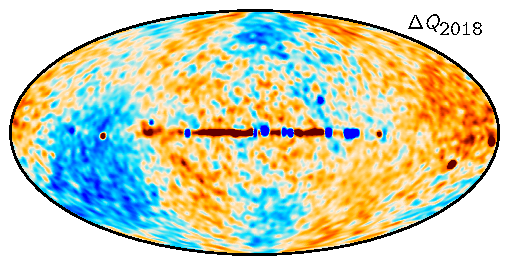
\includegraphics[width=\linewidth]{figures/diff_dpc_k_3deg_Q.pdf}\\
    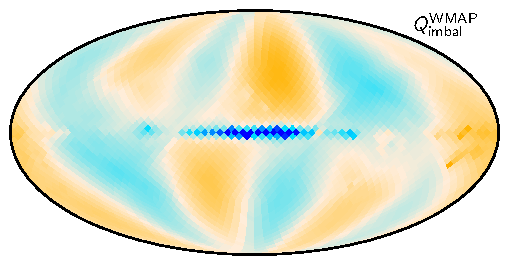
\includegraphics[width=\linewidth]{figures/wmap_loss_imbalance_template1_K1_v5_iqu_Q.pdf}\\
    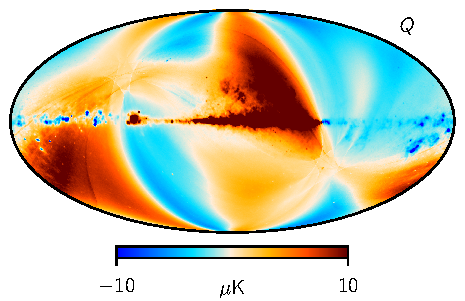
\includegraphics[width=\linewidth]{figures/LFI_gain_template_030_Q.pdf}
    \caption{(\emph{Top row}:) Stokes $Q$ difference map between the 30\,GHz \Planck\ 2018 map and the $K$-band 9-year \WMAP\ map, smoothed to a common resolution of $3^{\circ}$ FWHM, and the latter has been scaled by a factor of 0.495 to account for different center frequencies; see \citet{bp07} for further discussion. (\emph{Middle row}:) \WMAP\ transmission imbalance template \citep{jarosik2007}. (\emph{Bottom row}:) \Planck\ 30\,GHz gain residual template \citep{planck2016-l02}.}
    \label{fig:diff_30_k}
\end{figure}

\begin{figure}[t]
    \center
    \includegraphics[width=\linewidth]{figures/quiet_plane.pdf}
    \caption{Latitude-averaged Stokes $Q$-band differences between
      QUIET\ 43\,GHz and \WMAP\ $Q$-band (red) and between
      QUIET\ 43\,GHz and \Planck\ 2015 44\,GHz (blue) over the
      QUIET\ Galactic center field, evaluated over a latitude band
      around the Galactic plane of $|b| \leq 1\pdeg5$; reproduced from
      \citet{ruud:2015}. The colored regions indicate the absolute
      QUIET\ calibration uncertainty of $\pm$6$\,$\%. The dotted
      lines show the latitude-band-averaged \WMAP\ Q-band temperature
      amplitude scaled by a factor of $\pm 0.002$, providing a rough
      template for a 0.2\,\% temperature-to-polarization leakage in \Planck. The
      gray region marks an area in longitude $\pm 1\deg$ around the
      Galactic center within which all results are dominated by
      uncertainties in the foreground spectral index.}
    \label{fig:quiet}
\end{figure}

\subsection{Breaking degeneracies through joint analysis of complementary datasets}

The fundamental motivation for the \BP\ and \cosmoglobe\ projects derives directly from the experiences and insights gained within the \Planck\ project. Towards the end of that project, it became clear that the main limiting factor with respect to constraining large-scale CMB polarization comes neither from instrumental systematics nor astrophysical foreground modeling as such but rather from the interplay between the two\footnote{ \href{https://www.cosmos.esa.int/web/planck/lessons-learned} {\texttt{https://www.cosmos.esa.int/web/planck/lessons-learned}}}. As formulated in \citet{bp01},
\begin{quotation}
\ldots \emph{one cannot robustly characterize the astrophysical sky without
  knowing the properties of the instrument, and one cannot
  characterize the instrument without knowing the properties of the
  astrophysical sky}.
\end{quotation}

One demonstration of this ``chicken-and-egg'' problem is shown in Fig.~\ref{fig:diff_30_k}, reproduced from \citet{bp07}, where the top panel shows the Stokes $Q$ difference map between \Planck\ 2018 30\,GHz \citep{planck2016-l02} and \WMAP\ $K$-band \citep{bennett2012}, after scaling the latter by 0.495 to account for the spectral index of synchrotron emission. Here one can see coherent large-scale patterns that massively dominate over the random noise. The origin of these structures is well understood and can, to a considerable extent, be described by the sum of transmission imbalance uncertainties in \WMAP\ (middle row; \citealp{jarosik2007}) and gain uncertainties in \Planck\ (bottom row; \citealp{planck2016-l02}). Both the transmission imbalance and the gain estimation rely directly on knowledge about the CMB sky, while estimating the CMB sky relies on knowledge about the transmission imbalance and gain parameters. However, even though their physical origins are well understood, they are still exceedingly difficult to mitigate within each experiment individually, simply because the observation strategy of each experiment leaves them nearly blind to these particular modes. One of the solutions to this problem is to jointly analyze each experiment and use the information in one experiment to break the degeneracies in the other.

Such complementary information need not only come from expensive satellite missions but can also come from less expensive ground-based experiments. One example of this is depicted in Fig.~\ref{fig:quiet}, reproduced from \citet{ruud:2015}, which shows latitude-averaged polarization differences between the 43\,GHz QUIET\ map and the corresponding 9-year \WMAP\ (red curve) and \Planck\ 2015 (blue curve) maps. In this case, one can see an excess in \Planck\ with respect to QUIET\  outside $|b|<1^{\circ}$, while QUIET\ and \WMAP\ agree well. The most likely origin of this excess is bandpass-induced temperature-to-polarization leakage \citep{ruud:2015,bp09} in the \Planck\ map at the level of 0.2\,\% (dotted line), which is fully consistent with the quoted systematic error of this channel of $<$1\,\% \citep{planck2014-a04}. To reduce this systematic uncertainty below that achievable by \Planck\ alone, additional external information is required, and the deep and highly cross-linked Galactic plane measurements made by QUIET\ are precisely what is needed for this.

These are only two relevant examples, and many more could be listed. Nevertheless, such examples motivate our contention that in order to break instrumental and astrophysical degeneracies, all free parameters should be optimized jointly while simultaneously exploiting as many state-of-the-art complementary datasets as possible. As such, the analysis problem should be solved globally, both in a statistical and a research community sense. 

\subsection{The \BP\ data model and posterior distribution}
\label{sec:posterior}

\begin{table}[t]
  \begingroup
  \newdimen\tblskip \tblskip=5pt
  \caption{
    Resource overview for selected past, present, and future CMB
    experiments. Columns indicate experiment name, funding agency
    cost, collaboration lifetime (defined from
    proposal submission to publishing final paper), and number of
    collaborators as defined either as number of co-authors on a main
    paper or as the team size listed on the project web page.
  }
  \label{tab:resources}
  \nointerlineskip
  \vskip -3mm
  \footnotesize
  \setbox\tablebox=\vbox{
    \newdimen\digitwidth
    \setbox0=\hbox{\rm 0}
    \digitwidth=\wd0
    \catcode`*=\active
    \def*{\kern\digitwidth}
    %
    \newdimen\signwidth
    \setbox0=\hbox{-}
    \signwidth=\wd0
    \catcode`!=\active
    \def!{\kern\signwidth}
    %
 \halign{
      \hbox to 0.5cm{#\leaderfil}\tabskip 3em&
      \hfil#\hfil\tabskip 1em&
      \hfil#\hfil\tabskip 1em&
      \hfil#\hfil\tabskip 1em\cr
    \noalign{\doubleline}
    \omit\textsc{Experiment}\hfil&
    \omit\hfil\textsc{Cost (M\$)}\hfil&
    \omit\hfil\textsc{Mission lifetime (yrs)}\hfil&
      \omit$N_{\mathrm{coll}}$\hfil\cr
      \noalign{\vskip 4pt\hrule\vskip 4pt}
      ACT++ & \phantom{0}42\rlap{$^{\rm a}$}& >16 & 149\cr
      BICEP++ & \phantom{0}30\rlap{$^{\rm a}$}& >20 & \phantom{0}91\cr      
      C-BASS & \phantom{00}3\rlap{$^{\rm a}$}& >15 & \phantom{0}35\cr
      CLASS & \phantom{0}17\rlap{$^{\rm a}$}& >12 & \phantom{0}60\cr
      CMB-S4 & \phantom{?}600?\rlap{$^{\rm b}$}& \phantom{>?}10? & 385\cr
	\textit{LiteBIRD} & \phantom{?}300?\rlap{$^{\rm c}$}& \phantom{>?}18? & 186\cr                  
      \Planck\ & 770\rlap{$^{\rm d}$}& \phantom{>}24 & 400\cr
      POLARBEAR & \phantom{0}16\rlap{$^{\rm a}$}& >12 & \phantom{0}75\cr            
      QUIET & \phantom{00}6\rlap{$^{\rm a}$}& \phantom{>0}6 & \phantom{0}50\cr
      SPT & \phantom{0}60\rlap{$^{\rm a}$}& >17 & \phantom{0}64\cr                  
      \WMAP\ & 150\rlap{$^{\rm e}$} & \phantom{>}18 & \phantom{0}21\cr      
      \noalign{\vskip 4pt\hrule\vskip 5pt}}}
  \endPlancktable
  \tablenote {{\rm a}} NSF contributions only, as listed on \url{https://www.nsf.gov/awardsearch/}.\par
  \tablenote {{\rm b}} Projected total project cost as of 2019.\par
  \tablenote {{\rm c}} JAXA budget cap.\par  
  \tablenote {{\rm d}} Includes spacecraft, scientific payload,
  launch, and operations, according to
  \url{https://www.esa.int/esaSC/SEM9WJ0XDYD_0_spk.html} and assuming
  an exchange rate of 1.10 \texteuro/\$.\par 
  \tablenote {{\rm e}} Initial proposed budget according to \url{https://www.skyatnightmagazine.com}.\par  
  \endgroup
\end{table}

As a first proof-of-concept of this global analysis approach, the \BP\ collaboration \citep{bp01} was formed with the explicit goal of re-analyzing the \Planck\ LFI measurements. This data set represents a significant, but manageable challenge in terms of data volume and systematics complexity. Also, building on the experiences gained through the \Planck\ project, we chose to adopt standard Bayesian parameter estimation techniques for our computer codes because of their unique flexibility and fidelity in terms of systematic error propagation. In particular, in the interest of saving costs and development time, we chose the CMB Gibbs sampler called \commander\ \citep{eriksen:2004,eriksen2008,seljebotn:2019} as our starting point, which formed a cornerstone in the \Planck\ data analysis \citep{planck2016-l04,planck2016-l05,planck2016-l06}.

The most crucial component in any Bayesian analysis is a parametric model for the data, which may typically take the following symbolic form,
\begin{equation}
\d = \s(\omega) + \n,
\end{equation}
where $\d$ denotes a given dataset, $\s(\omega)$ is a signal model
with free parameters $\omega$, and $\n$ is noise. The posterior
distribution, which quantifies the probability distribution of
$\omega$ as constrained by $\d$, is given by Bayes' theorem,
\begin{equation}
  P(\omega\mid \d) = \frac{P(\d\mid \omega)P(\omega)}{P(\d)} \propto
  \mathcal{L}(\omega)P(\omega),
  \label{eq:jointpost}
\end{equation}
where $\mathcal{L}(\omega)\equiv P(\d\mid \omega)$ is called the
likelihood, and $P(\omega)$ is called the prior; $P(\d)$ is a
normalization constant that is irrelevant for our purposes. The
likelihood quantifies the constraining power of the actual data, while
the prior summarizes our pre-existing knowledge regarding $\omega$
before the analysis.

For the \Planck\ LFI analysis that is presented in a series of
companion papers, we have adopted a parametric model that takes the
following form,
\begin{equation}
  \begin{split}
    d_{j,t} = g_{j,t}&\P_{tp,j}\left[\B^{\mathrm{symm}}_{pp',j}\sum_{c}
      \M_{cj}(\beta_{p'}, \Dbp^{j})a^c_{p'}  + \B^{\mathrm{asymm}}_{pp',j}\left(s^{\mathrm{orb}}_{j,t}  
      + s^{\mathrm{fsl}}_{j,t}\right)\right] + \\
    + &s^{\mathrm{1\mathrm{Hz}}}_{j} + 
    n^{\mathrm{corr}}_{j,t} + n^{\mathrm{w}}_{j,t}.
  \end{split}
  \label{eq:todmodel}
\end{equation}
For the purposes of the current paper, the specific meaning of each symbol is irrelevant, and we, therefore, refer the interested reader to Sect.~7 in \citet{bp01} for complete details. Here it is sufficient to note that this expression represents an explicit parametric model of both the instrument, as quantified by $\{g, \P, \B, \Dbp, s^{\mathrm{fsl}}, n^{\mathrm{corr}}\}$, and the astrophysical sky as expressed by the sum over components $c$, which for \BP\ includes CMB, synchrotron, free-free, spinning and thermal dust emission, and compact sources.

It is important to note that this model is far richer than what \Planck\ LFI is able to constrain on its own. Simply by counting degrees of freedom alone, we immediately note that the sky model has five free component amplitude parameters per pixel, while the LFI data only provide three independent frequencies. Consequently, the model is massively degenerate, and the LFI data must be augmented with external data. This is done in the current \BP\ analysis by including the \textit{WMAP} 33--61\,GHz \citep{bennett2012}, \Planck\ HFI 353 and 857\,GHz \citep{planck2016-l03}, and Haslam 408\,MHz \citep{haslam1982} measurements in the form of pixelized frequency maps. The advantage of this is that the model is now reasonably well constrained -- but a major disadvantage is that these external pixelized sky maps may be associated with their own systematic errors that may compromise the final results. To fully exploit the strengths of each dataset in breaking degeneracies through joint analysis, one should ultimately start from raw TOD for all involved observations, and properly model all potential systematic effects. This is a main goal of the \cosmoglobe\ effort.

\subsection{Low-level systematics, data longevity,
  and cost optimization}

Whenever the signal-to-noise ratio of a given dataset increases, new systematic effects become important and must be modeled. This general observation also holds true for the CMB community, which currently targets signals at the nanokelvin level; even minuscule effects need to be accounted for at such low signal levels. This directly increases the importance of external data, as no planned experiment is able to measure all relevant effects internally at the required precision. More typically, each experiment focuses on one piece of the entire puzzle that it does particularly well for technological reasons and relies on other experiments to provide information regarding other free model parameters.

At the most basic level, the reason for this optimization is just a matter of cost and complexity. In particular, modern CMB experiments cost so much that it is unacceptable for funding agencies and taxpayers to repeatedly and needlessly measure the same quantities. To illustrate these costs, Table~\ref{tab:resources} provides an overview of well-known CMB experiments in terms of their financial and human resources. The columns show funding agency cost,\footnote{Most of the cost estimates are typically lower limits, as they are collected from public databases, and some contributions may be missing.} mission lifetime (in years from proposal to completion), number of authors of first main paper (as a proxy for scientist effort), and reference used for a cost estimate. Here we see that ground-based or sub-orbital experiments typically cost at least about \$10\,M and involve 20--50 people, while current and next-generation satellite experiments usually cost hundreds of millions of dollars and involve hundreds of people.

To achieve new transformative results in the future within realistic budget limits, these existing billion-euro investments must be optimally leveraged and re-used for all future experiments. For this to be possible, however, it is also vital that the systematic error budgets of the old datasets are consistent with the requirement of the new experiments. Unfortunately, this has traditionally been a prohibitive challenge for one simple reason: Until now, most CMB experiments have primarily published frequency maps or angular power spectra---that are static by nature---as their main products. Once the time-ordered data have been co-added into pixelized maps, it is no longer possible to account for a wide range of low-level systematic uncertainties, but only a very limited number of high-level uncertainties, such as white noise, correlated noise on large angular scales \citep{bennett2012,bp10}, a single absolute calibration factor \citep{planck2014-a10,bp07}, or symmetrized beam uncertainties \citep{planck2016-l05}. This significantly limits the use of legacy data for future analyses.

There are two noteworthy exceptions to this rule, though, namely \Planck\ and \WMAP. Both published their full uncalibrated time-ordered data as part of their legacy releases. Hence, the corresponding co-added frequency maps may, at least in principle, be continuously improved as new information and complementary datasets become available. However, it is also important to note that neither \Planck\ nor \WMAP\ released \emph{the data analysis pipelines} that were used to reduce the data.

That is problematic for at least two reasons. First, from a practical point of view, the lack of functional analysis pipelines makes it very difficult and time-consuming for external scientists to repeat and improve the original analyses. Even more problematic, however, is the fact that most modern data reduction pipelines typically employ a significant number of critical ancillary datasets, for instance, ADC correction tables or far-sidelobe models. Since these are only used during low-level processing, few external researchers ask for them. As a result, they may easily be forgotten during the last stages of the main collaboration work and sometimes even lost when the original production computer systems are discontinued.

We argue in this paper that the optimal -- if not only -- way to ensure full reproducibility and data longevity is to release a complete and functional data processing pipeline together with the raw data, parameter files, high-level products, and documentation. Furthermore, we also argue that such a complete release should be required and supported in terms of dedicated funding for all future CMB experiments by the respective agencies (ESA, NASA, JAXA, NSF, etc.). This is clearly also in the funding agencies' own interests, as it guarantees that their investments may be optimally leveraged in future work.

In addition to sharing data, it is also worth noting that sharing analysis tools may lead to cost optimization of any given new experiment. Indeed, establishing common analysis tools across the field will free up analysis funding that can be better spent on understanding the instrument, exploring ground-breaking theories, or deriving novel secondary science. An important pioneering CMB-related example of this is \healpix\ \citep{gorski2005}, which both defines a standard pixelization that facilities easy data sharing and comparison across experiments, and provides a wide range of state-of-the-art and user-friendly tools to operate on these data \citep[e.g.,][]{zonca2019}, all published under an Open Source license. In general, common software tools are highly beneficial for the science community, funding agencies, and taxpayers.

\subsection{Open Science: From \BP\ to \cosmoglobe}

An important goal for the \BP\ project was to develop and publicly release a complete end-to-end analysis pipeline for one of the essential datasets in contemporary CMB cosmology, namely the \Planck\ LFI data \citep{bp01}. The motivation for this was two-fold. The first aim was to resolve a few notable issues with the LFI data that remained unresolved at the end of the official \Planck\ mission, in particular related to the global estimation of the instrumental gain \citep{planck2016-l02,bp07}. However, this represents only a first step in a much larger process, as embodied within the \cosmoglobe\ program, whose goal is to develop a general low-level analysis pipeline that would be applicable to a much more comprehensive range of experiments -- legacy, current, and future -- and at the same time support \emph{joint} analysis of these.

The full scope of this project is massive. For this work to succeed in the long term, it must be firmly based on an Open Science foundation: While a small group of dedicated people may be able to re-analyze one experiment (as \BP\ has done for \Planck\ LFI), integrating a wide range of complementary experiments without community contributions is unfeasible for several reasons. First, some important datasets may be proprietary, and the original stakeholders must be leading the analysis for legal reasons alone. Second, the systematic properties of most datasets are quite complicated, and expert knowledge is usually essential to formulate and generalize the data model. Third, the sheer amount of work to be done effectively requires cost-sharing among all interested parties, recognizing the currently constrained funding environment most researchers experience daily.

Fortunately, a solid financial base for the initial phases of this work has been established through three separate but complementary EU-funded projects. First, an ERC Consolidator grant called \btoc\ (total budget of 2\,M\texteuro) supports the implementation of time-domain processing in \commander, as presented in the current paper suite. \btoc\ will continue to operate until 2023, and facilitate continued algorithm development activities for \textit{LiteBIRD}, SPIDER, and \textit{WMAP}. The second project is an H2020-funded COMPET-4 project called \BP\ (total budget of 1.5\,M\texteuro), for which the main goal is to re-process the \Planck\ LFI observations in a Bayesian setting. \BP\ ended formally on November 30th, 2020, and its results are currently being reported. The third project is called \cosmoglobe, an ERC Consolidator grant (total budget of 2\,M\texteuro). It aims to build an Open Science CMB analysis community around these tools and use this to derive a new state-of-the-art model of the radio, microwave, and sub-millimeter sky. \cosmoglobe\ started in 2019 and will support community-wide activities at least until 2024 based on current funding.

In general, \cosmoglobe\ will be a hub for which analysis of both time-ordered and map-domain data from different experiments can be integrated into a single framework. A critical goal of \cosmoglobe\ is to support scientists working on incorporating the data from their own experiments into the larger \cosmoglobe\ framework and thereby analyzing the data efficiently, robustly, and economically. For the casual user who might be primarily interested in what the microwave sky looks like at some specified frequency, \cosmoglobe\ will provide a state-of-the-art and user-friendly sky model. By allowing scientists easy access and configuration of their experiment in this framework, \cosmoglobe\ will become an integral tool for forecasting and planning for experiments.

With a functional codebase in hand, as demonstrated by the current LFI-based data release, we believe that the time is now right for all interested parties to get involved in this work and extend the framework according to their own needs. We anticipate that such contributions will most typically take one of two forms. The first is stand-alone projects, in which the external user simply downloads the software and data and performs some analysis without input from the greater community. In this case, the only formal obligation for the user is to publish all derived codes under an equally permissive software license as the one used for \BP\ (which in practice means a GNU General Public License (GPL)) and to acknowledge previous work through appropriate referencing.

The second mode of operation is active participation in the \cosmoglobe\ framework. In this case, an external user or project may request direct expert \cosmoglobe\ support, for instance, in the form of software development and data analysis assistance. That is then likely to increase the chance of success significantly. In exchange for the support, the external user or project must commit to publicly releasing the underlying data after some proprietary period, and all directly contributing \cosmoglobe\ collaborators must be offered co-authorship, in accordance with standard scientific practices. Required details can be specified in a Memorandum of Understanding (MoU) between the external party and the relevant \cosmoglobe\ participants before the work commences. \cosmoglobe\ is intended to be a platform for initiating and supporting mutually beneficial collaborations.

\section{Reproducibility survey, tools, and licensing}
\label{sec:reproducibility}

We now turn our attention to the practical aspects of how to build an Open Science-based foundation for this work and start by presenting the results from a small and informal user survey undertaken at the beginning of 2018. We then examine some of the latest developments on reproducibility in science in general. Next, we identify several tools and services that are available online and aim to provide solutions for reproducible science. Finally, we review the most popular licenses used for Open Source development. These issues cover a variety of topics that constitute the current state of the art in reproducibility and Open Science as of 2018--19, and we anticipate and recommend that similar surveys will be conducted at the start of any future project since developments in this field are very rapid, and new and better solutions continuously emerge.

\subsection{User survey}

At the beginning of the project, an anonymous online questionnaire containing more than 40 questions about demographics, occupational capacity, and reproducibility was circulated to collect feedback from the project participants and their external collaborators regarding the state of reproducibility in their day-to-day experiences. This questionnaire contained questions probing the respondents' level of working experience, familiarity with source control systems, backup and restore procedures used to safe keep their work, their coding expertise, operating systems in use, familiarity with virtual machines, familiarity with existing reproducibility frameworks, their participation and involvement in reproducing other papers or being asked for help reproducing their own work.

We received a total of 39 responses, among which 82\,\% of the respondents were male and 18\% female; the age of the participants was roughly equally split into the 25--30, 31--35, 35--40, and $>$\,45 years age groups. One-third of the respondents had been active in science for 4--8 years, another third for 9--15 years, and the final third for more than 15 years. Almost half were research fellows, while close to 20\,\% were professors.

56\,\% of the respondents were actively using a source code repository to store their work. The most popular source code control software used was \texttt{Git}, followed by \texttt{SVN}. On safekeeping of their work, 62\,\% responded that they keep personal backups on external hard disks, and 46\,\% said they used free online services to store own backups. In comparison, another 41\,\% said that they trust the backups already offered by their institution.

Regarding reproducibility, more than 80\,\% responded that they had recreated the work described in another paper. A total of 62\,\% did so because the methods used in the original paper were interesting and they wanted to know more about them; 60\,\% did so because they wanted to extend the work and produce further results; while 33\,\% did so because they found the original results to be suspicious and wanted to verify their validity. These reproducibility attempts were performed for 1--5 papers for 70\,\% of the respondents; for 6--15 papers for 20\,\% of the respondents; and for more than 15 papers for the remaining 10\,\% of the respondents. For each reproduced paper, 73\,\% claimed that they would do anything in their power to recreate the results of a given paper if it was important for their work, whereas 15\,\% claimed that they would spend up to 2--3 days trying to recreate it; 10\,\% claimed that they were willing to spend up to 1 week trying to get successful results.

As many as 97\,\% would first ask for assistance from colleagues in their attempts to recreate other papers, while 60\,\% would directly contact the original author/s asking for clarifications. From the participants who actually contacted the original authors, 68\,\% found that the author was helpful in assisting; 21\,\% claimed that the author's reply was ambiguous and/or unclear; while 5\,\% said that they never heard back from the original author.

Conversely, 51\,\% of the participants claimed that they had been contacted for help in recreating their own work; 43\,\% only once, and 24\,\% more than 10 separate times. Among these, 20\,\% of those contacted did not reply. From the ones that responded, 47\,\% spent only a few hours assisting, while another 43\,\% had communications that lasted several weeks until the issue was resolved. Of the participants who failed to respond to the queries for help, 60\,\% mentioned that the requests were trivial; 40\,\% said that they lacked free time at the time of the request; while other respondents noted that the requests were either unclear or insulting in nature, or that the work was partly covered by copyright or they were confidential.

A total of 26\,\% of the respondents said that they were willing to allocate one week extra to ensure that their work was reproducible; 37\,\% were willing to spend up to a couple of additional days; while 24\,\% were only willing to spend a few hours. The majority of the respondents, 78\,\%, said that they would like to have a reproducibility workflow\footnote{\textit{Reproducibility workflow} is the workflow that includes everything needed to make results reproducible,  starting from the version control system (e.g., \texttt{Git} or \texttt{SVN}) and finishing with data synchronization.}  embedded in their work. In comparison, only 10\,\% claimed otherwise. Smaller percentages said it depends on the work's nature or complexity.

Among the people who wanted to make their work reproducible, 54\,\% attempted to design a reproducibility workflow of their own, while the remaining 46\,\% searched online to find already established approaches. Among these, 56\,\% were unable to find a clear and easy-to-follow reproducibility workflow, and 46\,\% ended up just being a little more descriptive in the explanations provided in their paper; 25\,\% ended up asking other colleagues what they use to provide reproducibility in their papers; and 21\,\% simply gave up while not being able to find anything actionable.

The results of this survey should be taken with a grain of salt, in part due to selection effects, e.g., the fact that a scientist who values collaboration is more likely to respond to a survey on collaboration and reproducibility. Nevertheless, among the surveyed scientists, it is clear that reproducibility is an important component of their day-to-day work. Moreover, the fact that, among these collaboration-minded scientists, there are apparent deficiencies in easily-accessible and reproducible workflows indicates that there is ample room for improvement to support an effective Open Science ecosystem.


\subsection{Open Science development tools per 2018}

After the completion of the user survey reported above, we collected information regarding available tools that might be useful to strengthen the reproducibility aspects of the project. We found this exercise quite informative and helpful, and we highly recommend future collaborations to conduct similar meta-studies \emph{before} starting the data analysis work, as it is easy to get swamped with scientific problem solving once the main effort begins. We also note that the field moves very quickly, and the state-of-the-art is likely to be quite different only after a few years.

\subsubsection{Workflow definition tools versus integrated software}

We first considered the use of so-called ``workflow definition tools'' to organize the primary data model and Gibbs sampler discussed in Sect.~\ref{sec:posterior}. Such workflow managers help scientists define and execute a specific set of tasks, implemented by executing local (or sometimes remote) code, scripts, and other sub-workflows. Each component is only responsible for a small fragment of functionality. Therefore many pieces are working together in a pipeline to achieve the ultimate goal of the workflow, performing a useful task.

There have already been attempts at implementing and utilizing such tools in the CMB community. The most well-known example is the \texttt{ProC} workflow manager\footnote{\href{http://planck.mpa-garching.mpg.de/ProC/}
{\texttt{http://planck.mpa-garching.mpg.de/ProC/}}} developed by the Max Planck Institute of Astrophysics for the \Planck\ mission. Two popular Open Source and general-purpose tools are \texttt{Taverna}\footnote{\url{https://taverna.incubator.apache.org}} and \texttt{The Kepler Project}\footnote{\href{https://kepler-project.org/}
{\texttt{https://kepler-project.org/}}}.

The main advantage and attraction of such workflow managers is their ability to construct complex, flexible, and reproducible workflows based on well-defined components. At the same time, what makes these managers work is very strict interfaces between the different components. Unfortunately, this strictness adds significant additional burdens on the code developers, both in terms of a steep learning curve to be able to add new features and in terms of restricted flexibility to implement new solutions to unexpected problems; it is difficult to make substantial changes without breaking compatibility with already existing components. A second significant challenge is efficient memory management. Suppose the various pipeline components are written in different programming languages. In this case, one must either resort to data sharing through slow disks or spend great effort on highly non-trivial in-memory communication.

In general, our experience is that general-purpose workflow managers tend to be more practical for well-established and relatively quick routine tasks than for cutting-edge research that relies on high-performance computing. The most critical priority for our Bayesian analysis framework is computational speed, as a factor of six in runtime can make the difference between a two-month runtime (which is painful but doable) and one year (which is prohibitive). Optimal memory and disk management are, therefore, the key. The second most important priority is code flexibility, allowing developers to introduce changes needed to achieve their goals freely.

After careful consideration, we decided to drop the use of workflow managers, as the official \Planck\ Data Processing Centers (DPCs) did, to maintain optimal coding agility and flexibility. However, in contrast to the \Planck\ DPCs, we instead opted for developing the entire analysis pipeline within one single computer program called \commanderthree, to ensure optimal memory management and computational speed \citep{BP03}. Two important additional advantages of implementing the entire pipeline within a single code are that the whole collaboration naturally develops a common ``language'' and knowledge base that are helpful to discuss issues more efficiently, and it also minimizes duplication of effort.


\subsubsection{Online development services}

Another potentially useful class of tools is the so-called ``online development services''. These offer the possibility to perform all development work to be done online through the use of general-purpose web applications. Some of the major players in this area that we evaluated were \texttt{Open Science Framework}\footnote{\url{https://osf.io/}}, \texttt{Codeocean}\footnote{\url{https://codeocean.com/}}, and \texttt{Zenodo}\footnote{\url{https://zenodo.org/}}.

One of the major advantages of these services is that, by definition, all work is performed online. This facilitates very easy dissemination since results may be published in an Open Science manner literally in real-time. However, our evaluation is that they are also associated with three main disadvantages, mirroring the issues discussed in the previous section. First and foremost, online services typically impose a specific and inflexible work style that may not suit everybody in a large collaboration. Second, they have a significant learning curve that may be off-putting to many scientists with busy schedules. Third, depending on the plans offered by each provider, authors can easily run out of hosting space or online computational time, requiring them to update their accounts. While this may make financial sense from the side of the hosting companies, we consider this to be a big disadvantage for authors, just for reproducibility purposes alone. A solution like this might make sense for small projects, but the cost can become prohibitive for larger and heavier collaborations.

At their current stage of development, we, therefore, also decided to avoid the use of integrated online development services and instead leave each collaborator to choose their own development environment individually. We also note that most scientists are, by nature, quite independent-minded and do not necessarily respond well to being imposed on a specific development environment. However, if the available tools offered more obvious advantages, the situation might be different, and we definitely recommend future collaborations to perform a similar survey.


\subsubsection{Software repositories}

One class of software development tools that is critical for a large-scale Open Source effort is efficient \textit{revision control systems} (RCSs). This allows users to collaborate on the same computer program or scientific paper in real-time with a minimum of synchronization problems and is a cornerstone of modern software development. As noted above, 56\,\% of the user survey respondents already use at least one such system, with \texttt{Git} being the most popular.

At the beginning of the program, we quickly settled on \texttt{Git} as our main RCS, primarily because it was most widespread in our group, but also because we find that it handles merges and conflicts better than most competitors. The main question was then which (if any) common repository we should use. Three particularly well-known providers are \texttt{Bitbucket}\footnote{\url{https://bitbucket.org}}, \texttt{GitHub}\footnote{\url{https://github.com}}, and \texttt{GitLab}\footnote{\url{https://about.gitlab.com/}}.

One advantage of \texttt{GitLab} and \texttt{Bitbucket} is that they offer free private repositories in addition to public ones. This option might make them a better candidate for users who want to start their project as a private repository but switch to a fully public repository later on, closer to publication time. In addition, all three offer a full suite of online development tools, including bug/issues management, wiki pages, file hosting capabilities, and API access to hosted files.

Initially, we adopted \texttt{GitLab} as our main provider, primarily because it allows code to be run remotely on their web hosts. In addition, we considered that it might be helpful for small tasks, such as implementing online tools and calculators or automatically compiling paper drafts after each submission. However, it is important to note that this feature is only free for limited usage. Therefore, we have concluded it was not as useful as initially anticipated. Consequently, halfway through the project, we have switched to \texttt{GitHub} for our central software repository, simply because most people in our community already have accounts there and to avoid overhead by maintaining two separate accounts for most users.


\subsubsection{Open Source licenses}

When working in an Open Science setting, it is vital to protect the investments and interests of the various contributors and users. A critical aspect of this is licensing. Today, many Open Source licenses are in active use, and an important task for projects like \BP\ and \cosmoglobe\ is to choose the appropriate one for the work at hand. In this section, we provide a brief overview of licenses in the most common use today and discuss which one was chosen for our project, given the basic requirements that (1) our software should be Open Source; (2) all derivatives of this work should remain Open Source; and (3) our license should not contradict the licenses of any dependencies (\texttt{HEALPix}\footnote{\url{http://healpix.sourceforge.net} or \url{https://healpix.sourceforge.io}}, \texttt{FFTW3}\footnote{\url{https://www.fftw.org}}, etc.).

Although the term \textit{Open Source software} may be intuitively understood to be freely distributable, modifiable, and shareable code written by a single or a group of programmers, it is, in reality, more complex than it may seem at first glance. Generally speaking, when discussing software licenses, one needs to distinguish between several different aspects and concepts. The first aspect concerns basic distribution. On the most restricted side, \emph{proprietary software} is considered private property, and users are not allowed to share, study, change, or reverse engineer the provided software. A variation of this is called \emph{freeware}; in this case, the original software developer retains all rights, and the only difference is that end-users do not need to pay for the basic usage of a given program. \textit{Source available software} is software that allows users to view the source code but does not necessarily give the right to distribute, modify and/or install it on their machines. One example of such a license is the \textit{Commons Clause License}\footnote{\url{https://commonsclause.com/}}, which prohibits users from selling the software. Because of such restrictions, source available licenses are generally not considered to be Open Source. Next, \textit{Public Domain software} or ``unlicensed'' software is software that waives all the rights of copyright, trademark, or patent. Such software belongs to the ``public'' that uses it, and it can be freely distributed, modified, and/or sold without attribution to anyone. Examples of such licenses are \textit{Creative Commons} (CC0) and \textit{Unlicense}. During the course of history, experts have been arguing whether this type of license should be considered Open Source or not\footnote{Lawyer Lorence Rosen has written the essay titled ``Why the public domain isn't a license''—faced with strong opposition he has accepted that CC0 can be considered open-source.} even though they have many common features. Because of these disagreements, we also do not consider this license to be a proper Open Source license in the present work.

Moving on to what is considered proper Open Source software, \textit{free software} (FS), as defined by the \textit{Free Software Foundation}\footnote{\url{https://www.fsf.org/}} (FSF), is ``software that gives its users the freedom to run, copy, distribute, study, change and improve the software''.  According to a formal definition, the software is not considered free if it does not respect the following four essential freedoms:\footnote{\href{https://www.gnu.org/philosophy/free-sw.html}
{\texttt{https://www.gnu.org/philosophy/free-sw.html}}}

\textbfit{Freedom 0:} The freedom to run the program for any
purpose.

\textbfit{Freedom 1:} The freedom to study how the program works,
and change it so it does your computing as you wish. Access to the
source code is a precondition for this.

\textbfit{Freedom 2:} The freedom
to redistribute copies so you can help others.

\textbfit{Freedom 3:} The
freedom to distribute copies of your modified versions to others. By
doing this you can give the whole community a chance to benefit from
your changes. Access to the source code is a precondition for this.

Finally, \textit{Open Source licenses} are defined by the \textit{Open Source Initiative}\footnote{\url{https://opensource.org/licenses}} (OSI) and include licenses that ``allow the software to be freely used, modified, and shared'', and comply with ten distinctive criteria\footnote{\url{https://opensource.org/osd}} that concern (1) free redistribution; (2) source code; (3) derived works; (4) integrity of the author's source code; (5) no discrimination against persons or groups; (6) no discrimination against fields of endeavor; (7) distribution of license; (8) the license must not be specific to a product; (9) the license must not restrict other software; and (10) the license must be technology-neutral.

Both FS and OSI are considered to be Open Source with only subtle
differences.\footnote{These are more philosophical in nature. As
  Richard Stallman, the founder of GNU Project and FSF, stated: \textit{``The
  term `open source' software is used by some people to mean more or
  less the same category as free software\ldots The differences in
  extension of the category are small: nearly all free software is
  open source, and nearly all open source software is free.''}} While FS
is focused on the user's rights to use, modify and share the program,
OSI is focused on the source code being open with unrestricted
community driven
development.\footnote{\url{https://opensource.org/about}} Since the main
goal of the \cosmoglobe\ project is to build a community around a
common source code, this strongly suggest that the OSI definition is
most suitable for our purposes. However, looking at OSI's list of
the most popular and widely used licenses,\footnote{For the full list
  of open-source licenses, please visit:
  \newline
  \url{https://opensource.org/licenses/category}}
which includes GNU variants, we are going to use both definitions
interchangeably. 

\begin{figure*}[t]
    \center
    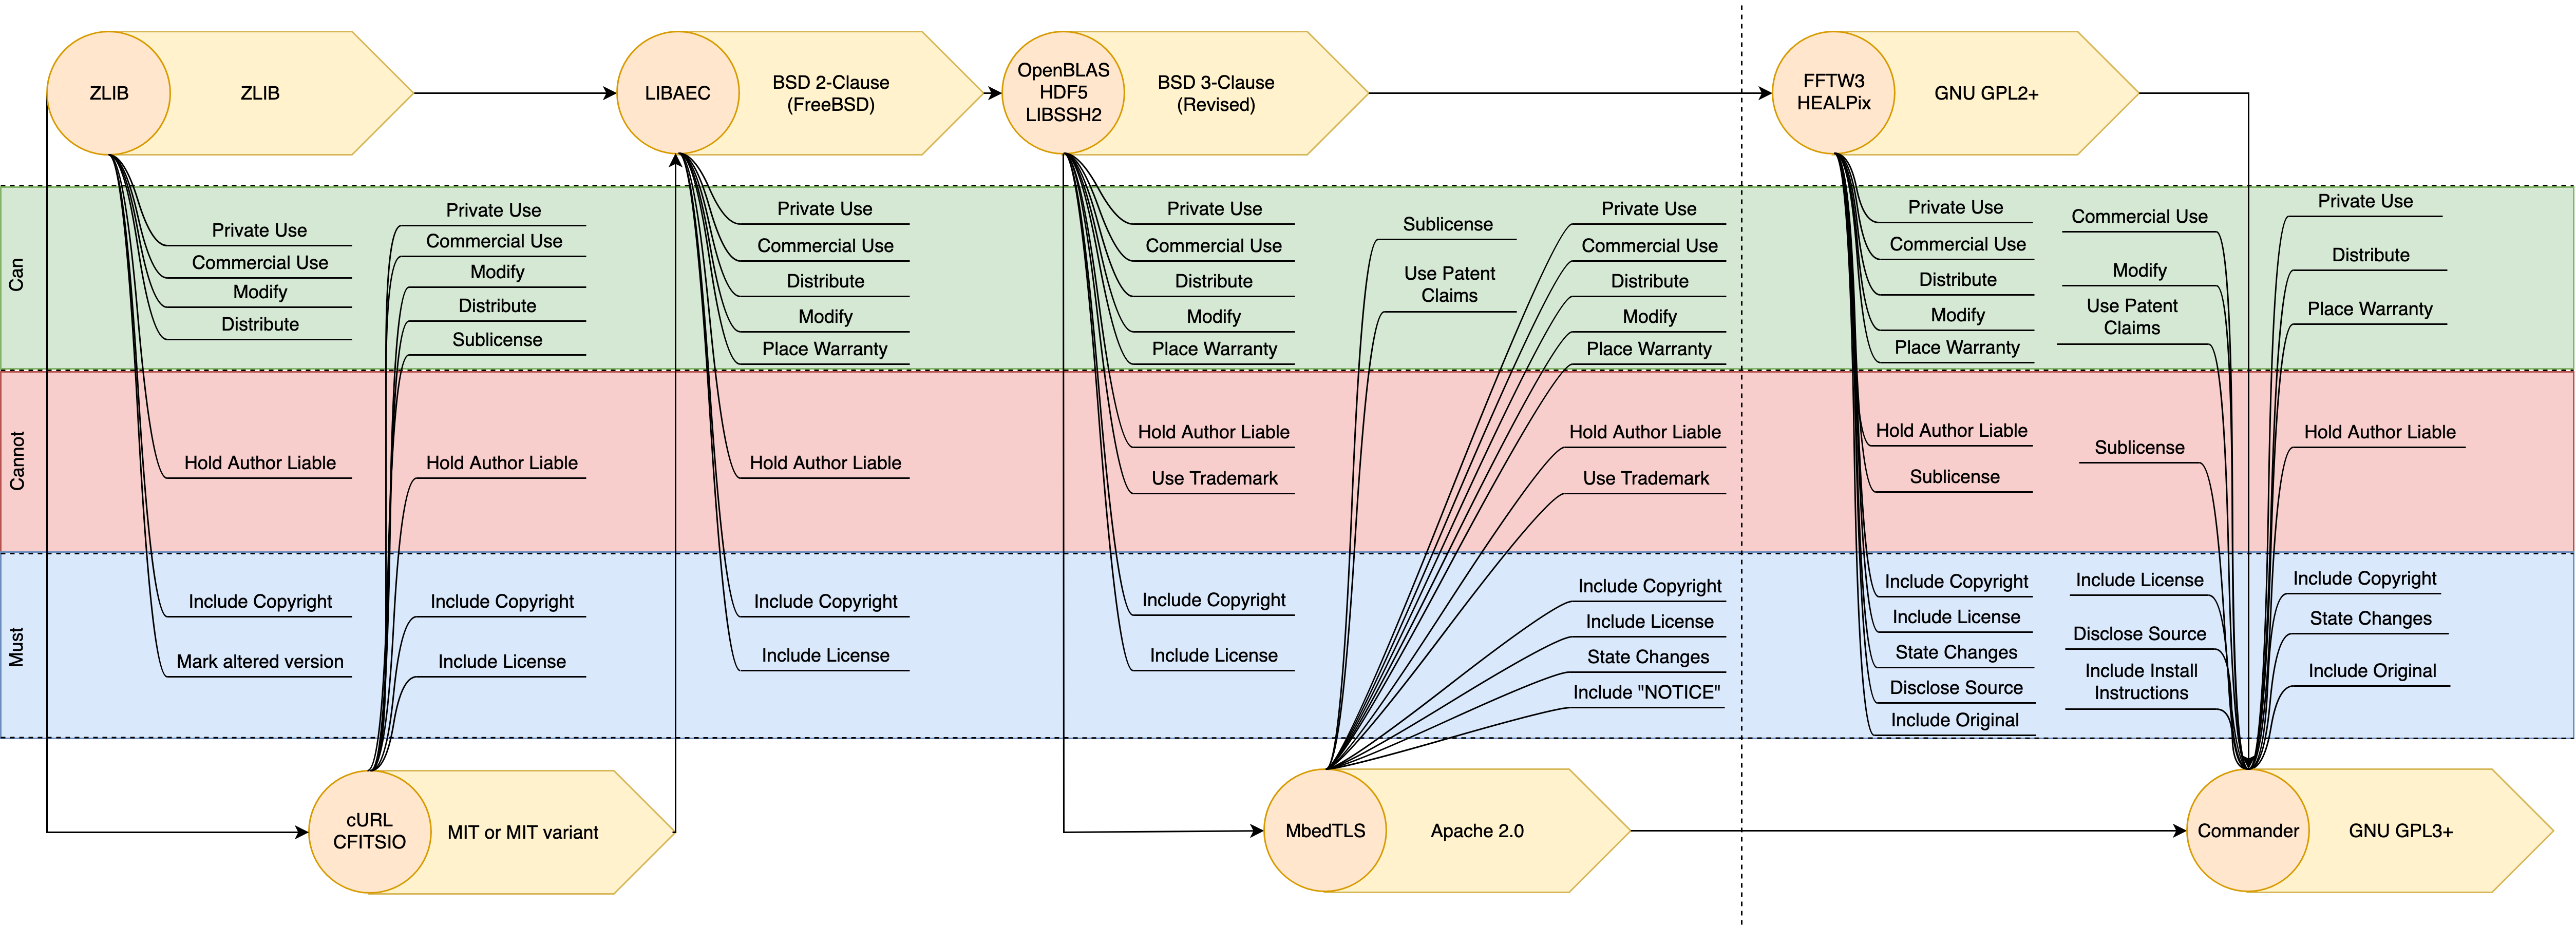
\includegraphics[width=\linewidth]{figures/Commander_Licenses_Diagram_v5.png}
    \caption{Licensing diagram
      for \commander\ and its dependencies,
      ordered from left to right according to increasingly specific
      licenses. Circles indicate libraries and codes, while rectangles
      show the licenses under which the particular library was
      issued. The dashed line divides the so-called permissive (i.e.,
      licenses that can be combined and used together with proprietary
      software) and restrictive licenses (i.e., licenses that enforce
      the source code to stay open for general public). This diagram 
      was derived from the David A. Wheeler's 
      \href{https://dwheeler.com/essays/floss-license-slide.html}{FLOSS License Slide}
      and the information provided on the \url{https://tldrlegal.com/}.} 
    \label{fig:licensing_diagram}
\end{figure*}

In order to select one of these OSI licenses, it is important to recognize that the \commander\ source code does not exist in a vacuum but rather depends directly and indirectly on a variety of different libraries, as visualized in Fig.~\ref{fig:licensing_diagram}. When one chooses the correct license for the project, the list of dependencies must be considered. Then, typically, the most specific one defines what is allowed for the new software. However, this is not always the case. For example, \texttt{cURL}\footnote{
  \url{https://github.com/curl/curl/blob/master/COPYING}} is based on the modified MIT license, but it may or may not be compiled with the support of \texttt{MbedTLS}\footnote{
  \url{https://github.com/ARMmbed/mbedtls/blob/development/LICENSE}}
and \texttt{LibSSH2}\footnote{
  \url{https://github.com/libssh2/libssh2/blob/master/COPYING}} that
rely on more complicated licenses. The same applies to, e.g.,
\texttt{CFITSIO}\footnote{\url{https://heasarc.gsfc.nasa.gov/docs/software/fitsio/c/f_user/node9.html}} which requires \texttt{ZLIB}\footnote{\url{https://www.zlib.net/zlib_license.html}} starting from version 4.0.0. A third important example is \commander\ itself, which may be compiled with Intel Parallel Studio and Intel Math Kernel Library (\texttt{MKL}), which are issued under one of Intel's proprietary licenses. We do not ship or install this library together with \commander\ in any way, and, thus, such a decision relies solely on the user's judgment.


Our understanding is that as long as one does not explicitly modify the source code of a library issued under a permissive license, the licenses can be used almost interchangeably. Generally, this does not apply to the restrictive ones. However, the GPL licenses are internally compatible as long as it includes a special line\footnote{ \textit{``(...) either version 2 of the License, or (at your option) any later version. (...)''}}  that explicitly states that the later version of the license can be used. In practice, this means that if a piece of software is issued under GPLv2 and not GPLv2+, then we cannot use it.  

All in all, the license adopted for \commander\ and \cosmoglobe\ cannot be more restrictive than the most permissive of these, which is set by the GPL2+ license adopted for \texttt{HEALPix}. In principle, the same applies to \texttt{FFTW3}, but if needed, this library could have been replaced with other FFT implementations. In contrast, \texttt{HEALPix} is in practice irreplaceable and therefore determines the license also for the current work. Consequently, our final choice is the GNU General Public License v3, as dictated by the diagram. Of course, for us, this is not only a matter of formality but also of preference; we \emph{want} this software to be and remain Open Source to protect the interests of everybody involved. Therefore, it is crucial for all future participants and developers of the \cosmoglobe\ framework to familiarize themselves with this license and determine whether this is acceptable for one's work and compliant with potential collaboration policies.

\section{Compilation support}
\label{sec:compilation_support}

The \commander\ software is primarily intended to be run on \texttt{Linux}-based \textit{High-Performance Computing} (HPC) clusters with basic \texttt{Fortran} and \texttt{MPI} compilers and libraries available and typically tens to thousands of computing cores. Beyond that, it does not impose any specific constraints on the computing platform, neither in the form of processor architecture (AMD, ARM, Cray, Intel, etc.)  nor compilers (GNU, Intel, PGI, etc.). At the same time, the code does depend on many external libraries, including \texttt{HEALPix}, \texttt{FFTW3}, \texttt{CAMB},\footnote{\url{https://camb.info/}} and \texttt{HDF5};\footnote{\url{https://www.hdfgroup.org}} for full
specification, see the online \commander\ documentation.\footnote{\url{https://cosmoglobe.github.io/Commander/}} The combination of many dependencies and a rich computing platform heterogeneity can, in general, represent a significant challenge and workload in terms of compilation and can be seriously off-putting to many users. Therefore, it is critical to make this process as simple and user-friendly as possible, and automated build systems play a key role in that work.


Build systems come in various flavors and combinations, which makes it non-trivial to choose one among many. As a result, there is no single ``best'' build system, but each has its advantages and disadvantages. Therefore, when selecting one specific system for \commander, we have considered seven different aspects listed in order of importance.

\textbfit{1) Free and Open-source}: \commander\ will not be a genuinely Open Source tool if the build system which installs it is itself not free and Open Source.

\textbfit{2) Cross-platform}: Although Linux was (and still is) the predominant operating system for modern HPC, there is currently a trend toward a more diverse landscape.\footnote{According to \href{https://www.top500.org/statistics/list/}{top500.org}, the share of non-Linux systems running the world's top HPC systems was 2.4\,\% in November 2010, 3.4\,\% in November 2014, 7\,\% in November 2019, and 16\,\% in November 2021.} In addition, Windows and Macintosh software dominate the PC and laptop market, and these systems are growing rapidly in power and can be used today for productive analysis. Hence, we require that the build system must allow us to compile and run \commander\ on any major operating system, including Linux, Windows, and MacOS.

\textbfit{3) Automation}: Many astrophysics departments operate today their own computing cluster. However, experience shows that there is often limited professional support for the installation, tuning, and maintenance of software and libraries. This work is often left to the scientists who want to run the code; Ph.D. students, postdocs, and professors. The installation procedure must therefore be both transparent and easy to use. Furthermore, it should be automated, i.e., the build system should be able to check for the existence of specific \commander\ dependency, and, if it doesn't find it on the host system, it should download, verify, compile, and install all missing dependencies, compile \commander\ itself, and link them all together.

\textbfit{4) Long-term support:} While Open Source projects have many advantages in current computing, they also tend to have one fundamental flaw: People tend to abandon them in favor of ``newer'' and ``better'' codes. This poses an obvious threat to a large and long-term project such as \cosmoglobe, which will require significant community-wide investments over many years. For this reason, the adopted build system should be mature and supported by a dedicated community. Proven stability is more important than cutting-edge.

\textbfit{5) Multi-language support:} The bulk of the \commander\ codebase consists of Fortran code, but there are many \texttt{Python} scripts and libraries written in the course of the development. In addition, there are also several \texttt{C++}-based modules that need to be compiled together with \commander, and other languages may become useful in the future. Therefore, the tool should have support for multiple languages used simultaneously in one project.

\textbfit{6) Minimal dependencies:} The build system should have as few dependencies as possible, and these should ideally either be already present in the system or easy to install from the source. Preferably, it should be a single binary or a piece of software.

\textbfit{7) IDE Integration:} While \textit{Integrated Development Enviroment} (IDE) support is not a strict requirement, it is certainly a nice bonus feature. In the present day and age, people are using a huge variety of IDEs that can perform syntax highlighting and code checking—having the same features available for the build system gives the programmer an advantage in terms of the code development speed.

With these points in mind, we now provide a survey of possible useful compilation support tools in current use and then describe the implementation chosen for \commander.

\subsection{Survey of automatic build systems}
\label{sec:build_systems_overview}

\subsubsection{Low-level build systems -- \texttt{Make}}
\texttt{Make} is a ``low-level'' build automation tool which uses special instruction files -- so-called \texttt{Makefiles} -- to build and install software from the source code. It has a variety of implementations, with perhaps, the most widespread one being GNU \texttt{Make} which is shipped together with most \texttt{Linux} and \texttt{Unix} distributions. In fact, \commander1 and \commander2 were solely built using \texttt{Make}. Its advantages are numerous: It is a standard Linux and Unix tool; it is widespread, and the majority of the scientific and open source community knows about it; it will not be deprecated in the foreseeable future since it has a solid community of maintainers; it as a support for a variety of languages such as \texttt{C}, \texttt{C++}, \texttt{Fortran}, \texttt{Java}, \texttt{Python}, etc.; it allows nested project structures; and, starting from version 3.0, it allows compilation using multiple processes.

However, it also has a few notable disadvantages. First, \texttt{Make} has a relatively obscure syntax and associated steep learning curve. Second, for large projects, such as \commander, the \texttt{Makefiles} tend to become very long and complex and increasingly hard to maintain. Finally, code compilation requires specific instructions for each particular compiler, OS, and architecture, making it a poor solution for cross-platform development. Despite these shortcomings, \texttt{Make} remains the most widespread build system in use today, and it has a firmly established user community. Taking into account both its flexibility and maturity, we have chosen \texttt{Make} as the primary low-level compilation system for \commander.

\subsubsection{High-level build system -- \texttt{CMake}}

Developed since 1999 under a BSD-3-Clause license, \texttt{CMake} is a ``meta'' or ``high-level'' build system that is used in conjunction with some other ``low-level'' build environments, for instance \texttt{Make}, \texttt{Ninja}, or \texttt{Microsoft Visual Studio}. \texttt{CMake} may be used to build a software project in a two-step process: First, \texttt{CMake} reads in a series of configuration files written in \texttt{CMake}'s own scripting language, called \texttt{CMakeLists.txt}, and use these to automatically produce a complete low-level build system configuration (e.g., \texttt{Makefiles}). Second, these files are used by the low-level native generator (e.g., \texttt{Make}) to actually compile and install the project.

\texttt{CMake} allows for flexible project structures. For instance, nested directory hierarchies and/or complex library dependencies do not pose a problem, as it can locate a variety of files and executables on the host system. Once such dependencies have been identified, the location data are stored inside a special file called \texttt{CMakeCache.txt} that can be manually tuned before the actual build. In addition, it has the functionality to download, verify, unpack and compile archives of missing libraries that utilize non-\texttt{CMake} build systems. Furthermore, cross-compilation is straightforward since \texttt{CMake} has extensive OS, language, and compiler support.\footnote{\url{https://cmake.org/documentation/}} Other important features include, but are not limited to, support for mathematical expressions; string, list, and file manipulation; conditions, loops, functions, and macros; and shell scripting.

Today, \texttt{CMake} is the de facto standard tool for \texttt{C++} project development,\footnote{According to a 2019 survey by \href{https://www.jetbrains.com/lp/devecosystem-2019/cpp/} {Jet Brains}, 42\,\% of \texttt{C++} projects use \texttt{CMake}; 33\,\% use \texttt{Makefiles}; 9\,\% use \texttt{Qmake}; 8\,\% use \texttt{Autotools}; and only 1\,\% use \texttt{SCons}. In addition, according to the \href{https://isocpp.org/blog/2021/04/results-summary-2021-annual-cpp-developer-survey-lite}{2021 Annual C++ Development Survey} roughly 80\,\% of all projects use \texttt{CMake} as one of their build systems.} and a variety of Open Source projects use \texttt{CMake} as its build system, including several \commander\ dependencies such as \texttt{CFITSIO}, \texttt{FFTW3}, and \texttt{HDF5}. Lastly, \texttt{CMake} has good support for IDE integration.

However, despite its many strengths, \texttt{CMake} is not perfect. The syntax has a pretty steep learning curve, and the source code may quickly become cumbersome and difficult to read. Also, there does not seem to be a universal approach, or even strict guidelines, for how to structure \texttt{CMake} code for large and complicated projects. Finally, the documentation is extensive but non-trivial to navigate and read for newcomers.

Based on its prevalence, mature community, rich feature set, and the fact that many \commander\ dependencies also use \texttt{CMake}, we have chosen this as our primary high-level build system, with \texttt{Make} as the corresponding low-level system. Specific details regarding the \commander\ \texttt{CMake} configuration is described in Sect.~\ref{sec:cmake}.

\subsubsection{Alternative build systems}

This section provides an overview of other competing systems that were explored during the initial phases of the project but ultimately not selected. However, several of these may be attractive candidates for future astrophysics and cosmology Open Source projects.

\textbfit{\texttt{Ninja}}\footnote{\href{https://ninja-build.org}{\texttt{https://ninja-build.org}}} is a low-level build system, similar to \texttt{Make}, specifically designed for speed. Like \texttt{Make}, it supports a variety of languages, platforms, compilers, and operating systems and, in fact, is meant to eventually replace \texttt{Make}. The main reason for not choosing \texttt{Ninja} over \texttt{Make} is simply the fact that it was designed to be used in combination with high-level build systems and not on its own. In addition, it is still in active development, and this carries a risk of higher -- and unnecessary -- development overheads for our purposes. This choice is likely to be revisited in the future when \texttt{Ninja} has proven itself further in terms of stability and user base.

\textbfit{\texttt{QMake}} or \texttt{makemake} is a build system created by the Qt Company which automates the creation of \texttt{Makefiles}, similar to \texttt{CMake}. It supports multiple platforms and can produce \texttt{Makefiles} tuned for specific operating systems. Although mostly used for \texttt{C++} projects, it can incorporate custom compilers (e.g., \texttt{gfortran}), and this allows it to work with \texttt{Fortran} source files. However, it lacks native support for non-\texttt{C++} languages, a natural alternative to \texttt{Make} build tools, and the ability to incorporate third-party libraries directly into the build.

\textbfit{\texttt{XMake}} is a lightweight build system that supports multiple languages, tool-chains, and platforms, and it can compile projects both directly and produce configuration files for low-level build systems such as \texttt{Make} or \texttt{Ninja}. However, native \texttt{Fortran} support was added as recently as July 2020 (in version 2.3.6), well after a system had to be chosen for the current \commander\ development. It is fast and has many IDE plug-ins.

\textbfit{GNU \texttt{Autotools}} is a GNU build system composed of several utility programs that are designed to make source code portable to many \texttt{Unix}-like Operating Systems. It is widely used by many free and Open Source projects, including several astrophysical and cosmology ones. In general, \texttt{Autotools} generate the distribution archive used to build programs. Once users obtain this package, they need to unpack it and run three simple and well-known commands -- \texttt{configure}, \texttt{make} and \texttt{make install} -- to compile and install the code using the facilities provided by their host systems. Such an approach, in theory, eliminates the need to install \texttt{Autotools} entirely, but, in practice, \texttt{Linux} distributions still have it with (sometimes) multiple versions installed, which adds to the confusion. Furthermore, a major drawback of \texttt{Autotools} is its complexity; it requires much experience and time to develop robust and user-friendly configuration files. For many future projects, we consider \texttt{CMake} to be a more accessible and user-friendly solution.

\textbfit{\texttt{Scons}} does not implement a new special-purpose and domain-specific language but rather utilizes specific \texttt{Python} scripts to build the projects. Thus, the only requirement is to have \texttt{Python} installed on the system, and this makes \texttt{Scons} cross-platform by default; any system that runs \texttt{Python} can install \texttt{Scons} using \texttt{Python}'s standard installation frameworks, \texttt{pip} or \texttt{conda}. MIT license, good multi-language support, reliance only on \texttt{Python}, and a rich feature set make it a tool worthy of exploring for new projects. A major shortcoming is that there does not appear to be a simple way of integrating other projects or dependencies into the build.

\textbfit{\texttt{Waf}} is another build system solely based on \texttt{Python}. Since \texttt{SCons} inspired \texttt{Waf}, both tools have many similar features: They rely exclusively on \texttt{Python}; are cross-platform; can automatically scan for project dependencies; and have support for multiple languages, including \texttt{C}, \texttt{C++} and \texttt{Fortran}. However, while \texttt{SCons} is older and therefore is used in more projects and has better documentation, \texttt{Waf} seems to be much faster and provides more user-friendly console output that makes it easier to debug. Additionally, it does not require a separate installation since the tool is designed to be shipped as part of the main project source code. Unfortunately, similar to \texttt{SCons}, there is no easy way to incorporate other projects into the build.

\textbfit{\texttt{Meson}} is the last \texttt{Python}-based tool considered here and is the closest \texttt{CMake} competitor we have found so far. It is similar to \texttt{CMake} in many (if not all) aspects, and both are meta-languages that compile the source code in a two-step process. However, while \texttt{CMake} uses \texttt{Make} by default, \texttt{Meson} uses \texttt{Ninja} instead; this makes \texttt{Meson} even faster in some cases. It is also an Open Source, cross-platform tool that supports multiple languages, including \texttt{Fortran}. In addition, nested hierarchies are not a problem, as well as the incorporation of other projects (both \texttt{Autotools}- and \texttt{CMake}-based) into the build.

\textbfit{Fortran Package Manager} or simply \texttt{fpm} is a relatively new\footnote{ Alpha version was released on \texttt{GitHub} in November 25, 2020.} initiative by the Fortran-Lang foundation\footnote{\href{https://fortran-lang.github.io/fpm/}{\texttt{https://fortran-lang.github.io/fpm/}}.} inspired by \texttt{Cargo}, the package manager for the \texttt{Rust} programming language. It is both a build system and a package manager that can build libraries and applications. In addition, it has native support for unit testing and can include other dependencies (e.g., from \texttt{Git}) into the project. While looking very promising, we considered that it was not ready for large-scale production at the time when the current project started. Still, this option should be revisited in the future.


\subsection{\texttt{CMake}-based compilation}
\label{sec:cmake}

As discussed above, we have adopted \texttt{CMake} and \texttt{Make}
as our high- and low-level build systems. In this section, we provide
an overview of the \commander-specific \texttt{CMake} configuration
and compilation procedure.

\begin{figure}[t]
\tikzstyle{every node}=[draw=black,thick,anchor=west]
\tikzstyle{selected}=[draw=red,fill=red!30]
\tikzstyle{optional}=[dashed,fill=gray!50]
\begin{center}
      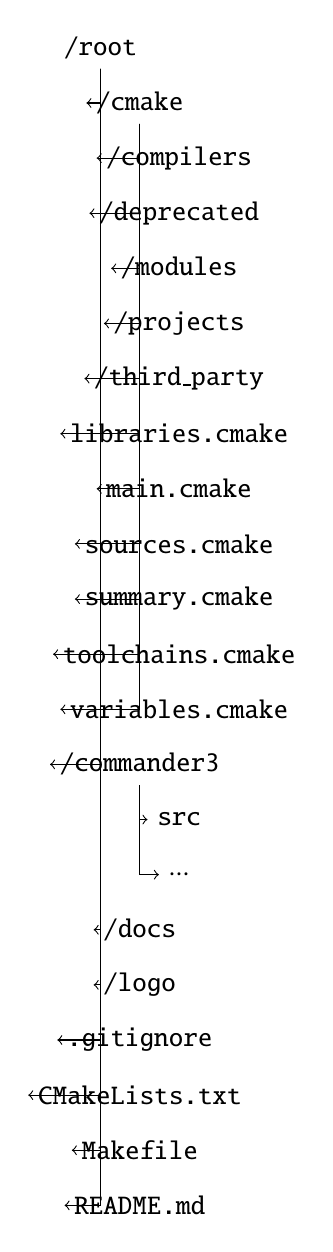
\begin{tikzpicture}[
                  grow via three points={one child at (0.5, -0.7) and
                              two children at (0.5, -0.7) and (0.5,-1.4)},
                  edge from parent path={[->](\tikzparentnode.south) |- (\tikzchildnode.west)}]
            \node {\texttt{/root}}
            child { node {\texttt{/cmake}}
                        child { node {\texttt{/compilers}} }
                        child { node {\texttt{/deprecated}} }
                        child { node {\texttt{/modules}} }
                        child { node {\texttt{/projects}} }
                        child { node {\texttt{/third\_party}} }
                        child { node {\texttt{libraries.cmake}} }
                        child { node {\texttt{main.cmake}} }
                        child { node {\texttt{sources.cmake}} }
                        child { node {\texttt{summary.cmake}} }
                        child { node {\texttt{toolchains.cmake}} }
                        child { node {\texttt{variables.cmake}} }
                        %child { node {...} }
                  }
            % adding these to make some space
            child [missing] {}
            child [missing] {}
            child [missing] {}
            child [missing] {}
            child [missing] {}
            child [missing] {}
            child [missing] {}
            child [missing] {}
            child [missing] {}
            child [missing] {}
            child [missing] {}
            child { node {\texttt{/commander3}}
                        child { node {\texttt{src}} }
                        child { node {...} }
                  }
            child [missing] {}
            child [missing] {}
            child { node {\texttt{/docs}}}
            child { node {\texttt{/logo}}}
            child { node {\texttt{.gitignore}}}
            child { node {\texttt{CMakeLists.txt}}}
            child { node {\texttt{Makefile}}}
            child { node {\texttt{README.md}}};
      \end{tikzpicture}
\end{center}
    \caption{Overview of \commander\ source code directory structure. 
    The \texttt{CMake}-scripts are inside the \texttt{cmake} directory. Here, 
    \texttt{compilers} contains compiler configurations; 
    \texttt{deprecated} contains deprecated code for convenience; 
    \texttt{modules} contains custom written \texttt{Find<Name>.cmake} modules; 
    \texttt{projects} contains configuration for all library subprojects; 
    \texttt{third\_party} contains \texttt{CMake} modules taken from other projects; 
    \texttt{libraries.cmake} handles general subprojects' configurations; 
    \texttt{sources.cmake} contains urls and various hashes for the subprojects; 
    \texttt{summary.cmake} module is for debug output of the final \texttt{CMake} configuration 
    on the screen; 
    \texttt{toolchains.cmake} module handles general compiler configuration; 
    \texttt{variables.cmake} has custom-defined variables available for to build \commander\
    as a single project; 
    \texttt{main.cmake} is there to mimic the logic of \texttt{C++}, \texttt{Fortran}, 
    \texttt{Python} etc. codes, and serves as an analogy to the ``entry point'' of the program.}
    \label{fig:source}
\end{figure}


\subsubsection{\commander-specific \texttt{CMake}-code organization}

Usually, when one is writing \texttt{CMake}-code for the project, each subdirectory has its own \texttt{CMakeLists.txt} file hence creating a tree-structure with the main \texttt{CMakeLists.txt} in the root of the project repository, while the ``leafs'' are in its respective subdirectories. However, since \commander\ has a substantial codebase already, we have decided to split the \texttt{Fortran} and \texttt{CMake} codes entirely. This allows for better navigation, makes the directory structure cleaner, and thus easier to maintain and expand. Furthermore, since the number of files involved in compiling \commander\ and its dependencies is significant, we have therefore adopted a so-called ``out-of-source'' build approach, as recommended by the \texttt{CMake} creators. In this organization, the source code and compiled build files are stored in separate locations. In our case, the source code itself is located inside the directory called \texttt{commander3}. In contrast, the binary folder is called \texttt{build}\footnote{It is worth noting that there is nothing special about this name, and the users can name the directory where the \texttt{CMake} build files will be stored in whatever way they prefer. However, the convention is to name it \texttt{build}.}, and it is usually created by the user inside the \texttt{root} directory. One advantage of out-of-source compilation is that the users can create whatever amount of \texttt{build} folders they want/require; thus, the same source code tree can be used to produce multiple binaries, corresponding, for instance, to different debug flags or CPU architectures.

All in all, the \commander\ source code directory structure is visualized in Fig.~\ref{fig:source}. In this figure, \texttt{root} represents the root folder of the project, created by the original \texttt{git clone} command; \texttt{cmake} contains all \texttt{CMake} related files; \texttt{commander3} contains all \commander\ related files; \texttt{docs} contains instructions on how to generate out-of-source documentation; \texttt{logo} contains \commander\ logos; \texttt{.gitignore} is a \texttt{git} version control file; \texttt{CMakeLists.txt} is the top level \texttt{CMake} configuration file, which serves as the starting point for the compilation process; \texttt{Makefile} is a traditional-style \texttt{Makefile} that may be used to compile \commanderthree\ without \texttt{CMake}; and \texttt{README.md} describes the project on \texttt{GitHub}.


\subsubsection{\commander\ \texttt{CMake} workflow}
\label{sec:cmake-code-organization}

\begin{figure*}[t]
      \center
      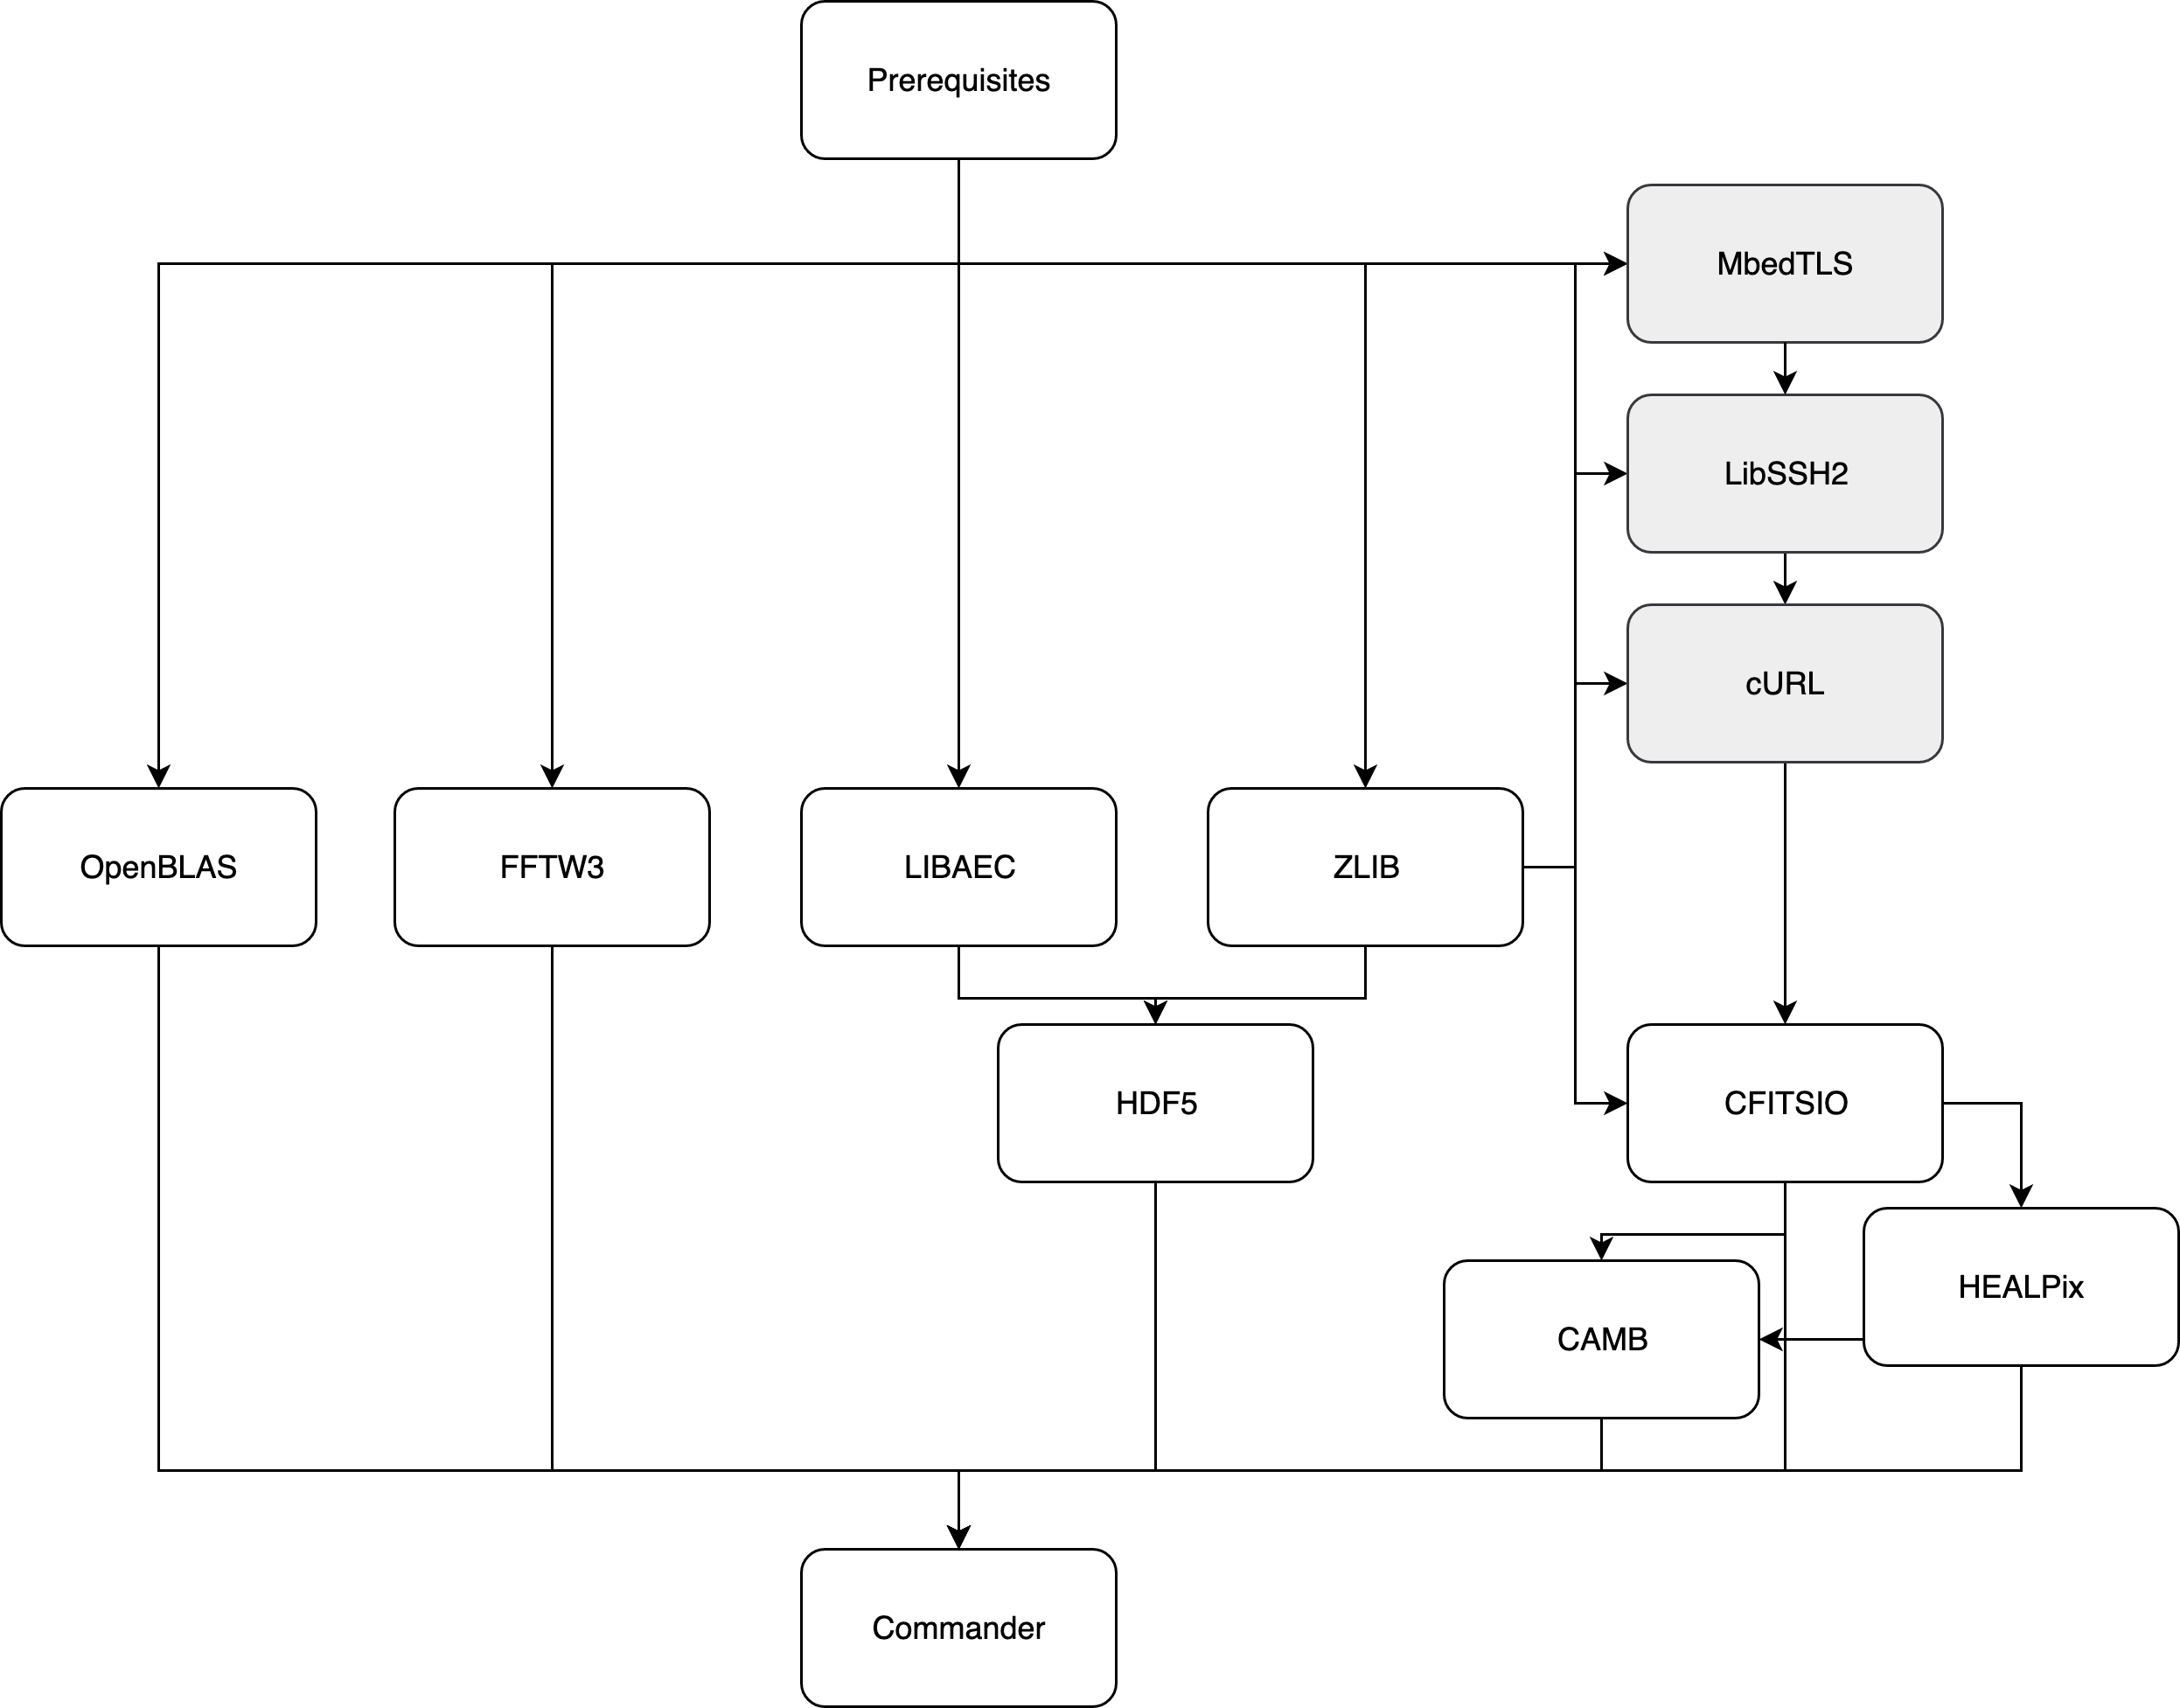
\includegraphics[scale=0.75]{figures/Commander_CMake_workflow.png}
      \caption{An example of the \texttt{CMake} \commander\ workflow. 
      The arrows represent the dependence and the linking, while the libraries 
      on the same level will be compiled in parallel. The libraries in grey are 
      optional dependencies. For example, \texttt{HDF5} is dependent on both \texttt{ZLIB} and \texttt{LIBAEC}. 
      The same goes for \texttt{CFITSIO} which may (or may not) be compiled with \texttt{cURL} 
      support depending on the user's preference. Since \texttt{cURL} is dependent on 
      a bunch of other libraries they also need to be incorporated into the build 
      even though \commander\ does not require them explicitly. 
      }
      \label{fig:cmake-workflow}
\end{figure*}


The \texttt{CMake} process works as follows. First, the host system is scanned, and the present/missing  libraries are registered inside \texttt{CMakeCache.txt} and other auto-produced files. Then, once the configure step is done and the user has issued the build command, \texttt{CMake} downloads, configures, compiles, and installs the missing dependencies and, together with the ones identified as available, it links all libraries to the compiled \commander.

The \texttt{CMake} module that enables this behavior is called \texttt{ExternalProject}, and its primary purpose is to facilitate downloading and installation of dependencies that are not an internal part of the main project. In this way, the \commander\ dependencies are treated as entirely independent entities. Such isolation allows the build to be performed in the same way on different platforms, with utterly different build settings (e.g., compiler flags) and/or with a completely different build system (e.g., \texttt{Autotools}). Under the hood, it defines the set of so-called targets, each representing a particular step in the build process of an external project. These steps are then collected under a unified name (in our case, a sub-project name), used later in the code. \texttt{CMake} also remembers information about each performed step, which, if executed successfully, will not be repeated. This allows us to compile all dependencies only once for different \commander\ build types. An essential feature for debugging this process (if and when something fails) is the \texttt{CMake} logs, which are stored in \texttt{/usr/local/logs}\footnote{The location can be changed by using defined \texttt{CMAKE\_LOG\_DIR} variable during the configuration process. We refer the interested reader to \commander\ documentation for further details.}.

Command-line arguments determine compiler selection during the scan phase. For instance, \texttt{-DCMAKE\_Fortran\_COMPILER=ifort} tells \texttt{CMake} to use the Intel \texttt{ifort} compiler. Then, for the most common compilers default optimization flags are defined per (sub-)project in a configuration file called \texttt{cmake/projects/{<project\_name>}.cmake}. When installing this software on a new system with a new, unknown to \commander\, compiler, these are the configuration files that most likely need to be updated.

Based on the initial system scan and user-specified compilation instructions, \texttt{CMake} proceeds with the following steps for each dependency and for the main \commander\ source (the two first steps are skipped in the latter case):

\textbfit{Download:} The project is downloaded via external links in the form of \texttt{.zip} or \texttt{.tar.gz} archives, or directly from \texttt{Git} repositories. We use \texttt{MD5} hashes whenever possible to ensure that the correct library versions are downloaded.

\textbfit{Update/Patch:} This step applies potential patches to the downloaded archive or, in the case of \texttt{Git}, brings the project up to date. In cases where we download the release versions of the packages, we skip this step.

\textbfit{Configure:} This step can use \texttt{CMake} and other build tools alike, depending on the preferences of the authors of the original dependency. In our case, most libraries use \texttt{Autoconfig} scripts and \texttt{Makefile} to compile.

\textbfit{Build:} In this stage, we use the default build tool as in the rest of the project.

\textbfit{Install:} The subproject is installed to a local directory specified by the user during the \texttt{CMake} configuration stage. It is worth noting that not all projects (e.g., \texttt{HEALPix}) support an explicit install command. We simply copy the compiled binaries and libraries into the specified directory in these cases.

These steps can either be sequential or parallel. In the former case,  each library is built sequentially, while the latter allows some libraries to be built in parallel. This idea is illustrated in  Fig.~\ref{fig:cmake-workflow}. It is important to note that this is not the only the way to compile \commander since \texttt{OpenBLAS}  can be substituted for, e.g., Intel \texttt{MKL}, which will be detected by \texttt{CMake} if present. 

\subsubsection{Installation regimes}
\label{cmake-installation-regimes}

\texttt{CMake} has various build types defined by default that allows for different optimization categories. We are calling these ``installation regimes'' with four of these currently supported:

\texttt{Release:} Builds \commander\ with the most aggressive optimization flags enabled, tuned for each specific compiler and platform. At the time of writing this paper, only Intel and GNU compilers were supported.

\texttt{Debug:} Builds the \commander\ executable without any optimization, but with debug symbols.

\texttt{RelWithDebInfo:} (``Release With Debug Information''). A compromise between the two above, building the \commander\ binary with less aggressive optimizations and with debug symbols.

\texttt{MinSizeRel:} (``Minimal Size Release''). Builds the \commander\ executable with optimizations that do not increase object code size. However, as the current software targets HPCs with ample disk space, this feature is not used frequently, and it is also accordingly not thoroughly tested.

While we have defined \texttt{RelWithDebInfo} to be the default one, the installation regime is determined by the user and his/her needs and can be changed via specifying \texttt{CMAKE\_BUILD\_TYPE} variable in the command line. In general, all external libraries are produced in  \texttt{Release} format with all optimization flags enabled. This can, however, be changed on a case-by-case basis by editing the \texttt{CMake}  source files mentioned above.


\section{Documentation, QuickStart guide, and accessibility tools}
\label{sec:bp_reproducibility}

For an Open Science project to succeed and continue to grow, making the source code and the data open to the general public is not sufficient. It is also critical that the framework is easy to use and adapt from the user’s perspective. Therefore, in this section, we provide a QuickStart guide to the \commander\ documentation and compilation, as well as discuss some valuable tools that make it easy for new users to get “up-to-speed” quickly. We note, however, that this is a continuous work-in-progress; thus, the section is only intended to give a snapshot of the situation at the time of publication.

While the \cosmoglobe\ framework is designed to simultaneously handle data from different experiments, it is helpful to consider the specific \BP\ pre-processing and analysis pipeline in greater detail, as this will typically serve as a point of reference for most users, whether they want to reproduce the LFI work or generalize the framework to other datasets. In the following, we, therefore, give an overview of the \BP\ installation procedure, but note that most of these steps will be identical for any \commander-based analysis.

\subsection{Online documentation}
\label{sec:docs}

The documentation for the \BP\ pipeline and \commander\ are currently available on the \commander\ documentation page of the official \cosmoglobe\ \texttt{GitHub} repository\footnote{\url{https://github.com/Cosmoglobe}}. It consists of five main sections, namely (1) Overview (2) QuickStart and installation guide; (3) The \commander\ parameter file; (4) File formats; and (5) Frequently asked questions.

Due to the dynamic nature of the \commander\ and \cosmoglobe\ projects, this documentation will continually evolve with the addition of new features or experimental datasets. Hence, active participation by the community is essential for its maintenance and expansion. Relatedly, it is also worth noting that because of the high \commander\ development rate, sometimes developers forget to document newly added parameters, and the documentation then becomes outdated. When this happens, the code may request parameters that are not explicitly mentioned anywhere. In these cases, we strongly recommend that the external user notifies the core developers by opening a \texttt{GitHub} issue -- or, better yet, corrects the documentation and submits the improved version in the form of a \texttt{pull request}.

\subsection{\BP\ QuickStart guide}
\label{sec:quickstart}

In the ideal case, installing the \BP\ analysis framework can be done
in four simple steps:
{\small
\begin{verbatim}
> git clone https://github.com/Cosmoglobe/Commander.git 
> mkdir Commander/build && cd Commander/build
> cmake -DCMAKE_INSTALL_PREFIX=$HOME/local \
        -DCMAKE_C_COMPILER=icc \
        -DCMAKE_CXX_COMPILER=icpc \
        -DCMAKE_Fortran_COMPILER=ifort \
        -DMPI_C_COMPILER=mpiicc \
        -DMPI_CXX_COMPILER=mpiicpc \
        -DMPI_Fortran_COMPILER=mpiifort \
        ..
> cmake --build . --target install -j 8
\end{verbatim}}
\noindent The first line downloads the \commander\ from the official \texttt{Git} repository, while the second line creates the aforementioned \texttt{build} directory in which compiled binaries and libraries will be stored. The third line collects information regarding the system and auto-generates \texttt{Makefile}s inside \texttt{build}. Finally, the last line downloads any potentially missing external dependencies and compiles both these and the main source code\footnote{After installing \commander, the user needs to update the shell to point out the location of the recently installed \texttt{HEALPix} library. This is done by \texttt{export}ing the \texttt{HEALPIX} variable inside \texttt{.bashrc} (or similar file).}. The whole process typically takes less than 10 minutes. We have used Intel compilers in this example, but GNU ones have also been successfully tested.

\begin{figure*}
      \center
      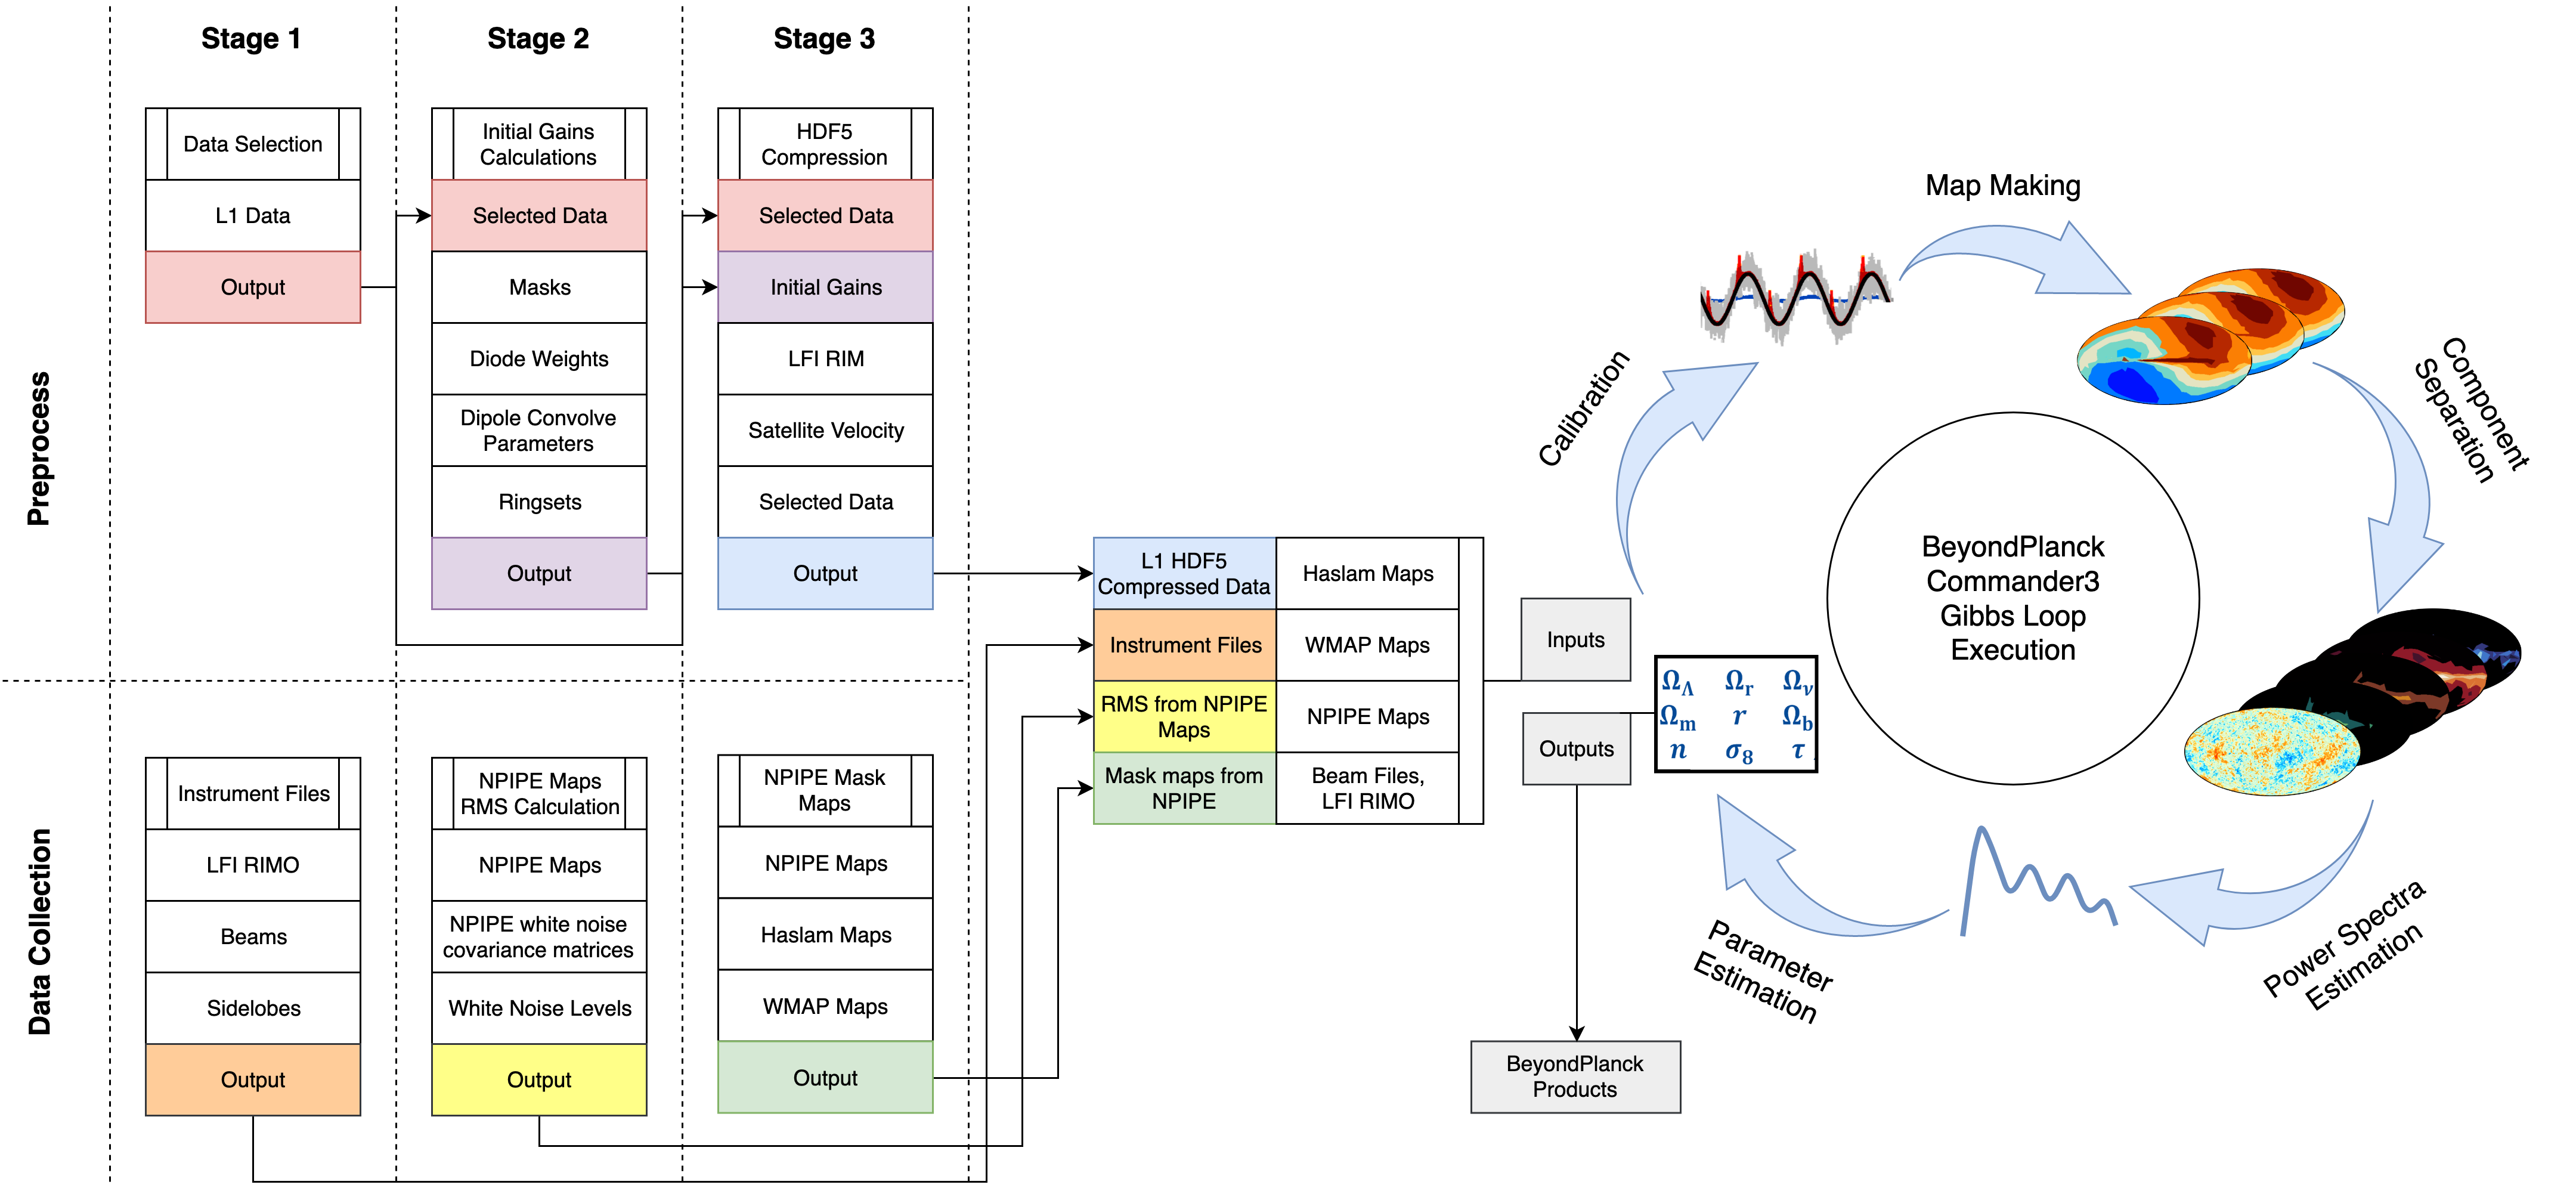
\includegraphics[width=18.5cm]{figures/bp_pipeline_reworked_v3.png}
      \caption{Schematic overview of the \BP\ pipeline pre-processing
        and initialization stages, along with all the input files
        required for each particular stage.}\label{fig:bp_pipeline_stages}
\end{figure*}

Once \commander\ is installed, the second step is to download the required input data. The number of different files required for a complete \BP\ run can be somewhat intimidating at first sight. To solve the problem, we have implemented a small \texttt{Python} utility called \texttt{bp} that helps new users to download all required data with a single command:

\begin{verbatim}
> bp download all
\end{verbatim}
\noindent This creates a complete directory structure with all required inputs, which amounts to more than 1\,TB of data. With a modest download speed of 10\,MB/s, this can take some time before completion. The tool also supports downloading individual sub-directories in case the user only requires a subset of the total data.

The third step is to edit the \commander\ parameter file. As described by \citet{BP03} and in the \commander\ documentation, this is a human-readable ASCII file. It is the step with the steepest learning curve in the process, as the number of \commander\ parameters is quite significant, and a typical parameter file spans several thousands of lines. To address the issue, we have enabled support for the nested include statements allowing for rarely used parameters to be hidden from the user. The downside of this approach is that the special environment variable should be defined in the user’s shell\footnote{It is called \texttt{COMMANDER\_PARAMS\_DEFAULT}, and it should point to the \texttt{<commander\_root>/commander3/parameter\_files/defaults} inside \texttt{.bashrc} (or other shell files if applicable.)} for everything to work. Even more so, although very helpful in most cases, such abstraction can still lead to difficult-to-debug errors and become a potential time spender since it requires considerable experience to debug \commander\ parameter files efficiently. A good strategy, in this case, is to start with a well-tested case (such as the final \BP\ parameter file) and only make a few changes between each test run, carefully visually inspecting all outputs at each step while gradually building intuition regarding the code outputs.

The fourth and final step is to actually run the code, which is
typically done through an \texttt{MPI} runtime environment:
\begin{verbatim}
> mpirun -n {ncore} path/to/commander param.txt
\end{verbatim}
The runtime for a given job varies wildly depending on the parameter file and computing facilities. Still, for the default \BP\ parameter file and a 128-core cluster, it takes about 1 hour and 40 minutes to produce one single sample \citep{BP03}. For a full Monte Carlo posterior exploration that requires thousands of samples, the end-to-end wall-time is typically on the order of months.

This QuickStart guide represents the ideal case where everything works out of the box. At the time of writing this paper, we estimated that the framework had been successfully installed on at least 20 independent computer systems -- and, unfortunately, the default process outlined above worked without modifications in no more than half of these. In the remaining cases, various issues popped up because of compiler idiosyncrasies, missing (or wrong version of) system utilities, insufficient user permissions or disk space, etc. To solve such issues when they arise and improve the current tools, it is vital to have a deeper understanding of all parts of the process, which is the main topic of the rest of the section.

\subsection{\BP\ pre-processing and initialization}
\label{sec:pipeline}

To understand the whole \BP\ analysis process, it is helpful to take a high-level look at the entire pipeline. This is schematically illustrated in Fig.~\ref{fig:bp_pipeline_stages}. The heart of this pipeline is the \commanderthree\ execution, discussed in the previous section and illustrated here by the rightmost analysis loop. This is where the actual posterior sampling takes place (see Sect.~\ref{sec:posterior}), and it is implemented in terms of a $\sim$\,60\,000 line \texttt{Fortran} code, as described by \citet{BP03}

However, \commander\ requires a significant number of input data objects in order to run, as illustrated by the various small boxes to the left in the figure. These include (1) the raw \Planck\ LFI Level-1 data (light blue box; \citealp{planck2016-l02}); (2) a so-called ``instrument file'' (orange box); (3) external and ancillary data that need no pre-processing (white boxes); and (4) external or ancillary data that do need slight preprocessing to conform with \commander\ conventions (colored boxes).

Going through these in order of low to high complexity, the white boxes represent external sky maps and ancillary data that may be used directly in their original forms. These include the frequency maps from \Planck\ HFI, \WMAP, and Haslam 408\,MHz, and various instrument characterization such as beam files and the \Planck\ LFI Reduced Instrument Model (RIMO). In many cases, these may be simply downloaded directly from external repositories, such as the \Planck\ Legacy Archive\footnote{\url{https://pla.esac.esa.int/}} or LAMBDA\footnote{\url{https://lambda.gsfc.nasa.gov}}, and inserted into \commander\ in their original form.

However, some information needs to be slightly pre-processed to match the format expected by the \commander. One example is the white noise specification per frequency band (yellow boxes), for which \commander\ expects the user to provide a standard deviation per pixel, whereas the official \Planck\ products provide a per-pixel $3\times 3$ covariance matrix. As such, the external user needs to reformat the \Planck\ format into the \commander\ format (or, better yet, implement support for the native \Planck\ format directly into \commander, and submit a \texttt{Git} pull request).

Another important example is masks (green boxes), which are used at various stages during the \commander\ processing. These may be defined differently whether one is considering correlated noise, gain, bandpass, foreground, or CMB estimation \citep[e.g.,][]{bp06,bp07,bp11,bp12,BP13,bp14}. These masks are typically based both on external sky maps (e.g., \Planck\ HFI or \WMAP) and internal results from a previous \commander\ iteration (e.g., $\chi^2$ maps), and properly optimizing these is an important (and non-trivial) task for any \commander\ user.

The third data collection box represents the so-called \commander\ instrument file. This plays a similar role as the RIMO in \Planck and contains detailed instrument information for a given frequency channel and detector. This includes objects that are general for all detectors, such as bandpasses and beams \citep{bp08,bp09}, but also instrument-specific objects such as ADC correction tables \citep{bp25}.

However, the most significant and crucial pre-processing step is the preparation of the actual raw time-ordered data, as indicated by the three ``Preprocess'' stages. These data are stored in compressed \texttt{HDF5} files \citep{BP03}, and include everything from raw detector readouts, pointing, flags, and satellite velocity to initial gain and noise estimates per \Planck\ pointing period.

To improve both user-friendliness and reproducibility in each of the above steps, it is useful to define scripts that perform all these tasks for the user. Within the \commander\ repository, we have therefore provided a series of (primarily \texttt{Python}) scripts that perform each of these operations, from mask and instrument file generation to full Level-1 data processing. These are intended to serve as useful starting points for users who seek to reproduce the current \BP\ LFI processing and for users who want to analyze a completely new dataset with the same framework. If so, it would be greatly appreciated if the new scripts are also committed to the existing repository as part of the community-driven Open Source activities.

Before concluding this section, it is worth noting that \commander\ has, in general, very few means of validating a given input data product. If, say, some instrument specification or compressed \texttt{HDF} files are inter-mixed, there is no automatic way for the algorithm to discover this except through visual inspection of the final results and goodness-of-fit statistics. Furthermore, such parameter file errors are likely among the most common and time-consuming errors made when running this code. For most analyses, it is, therefore, useful to start with the set of well-tested parameter and input files provided in the \commander\ repository \citep{BP03}, which includes individual parameter files for a wide range of common datasets (\Planck\ LFI and HFI, \WMAP, Haslam 408\,MHz, etc.) and astrophysical components (CMB, synchrotron, thermal dust emission, etc.). These may be used as ``building blocks'' when constructing a new analysis configuration.


\subsection{Docker environment for user-friendly data access and code exploration}

We provide a precompiled \texttt{Ubuntu}-based \texttt{Docker} image for users who are not interested in computationally expensive analyses like \BP\ but simply want to run \commander\ on a small dataset for which computational efficiency is not paramount. This self-contained operating-system-level virtual container can be run on any OS (\texttt{Mac}, \texttt{Windows}, \texttt{Linux}, etc.), and all dependencies are maintained within the \texttt{Docker} image itself. Running \commander\ in this mode amounts to one single command line:
{\small
\begin{verbatim}
> docker run -it \
  -v {input_dir}:{input_dir} \
  -v {output_dir}:/output \
  registry.gitlab.com/beyondplanck/r13y-helper/cm3 \
  commander3 {parameter file}
\end{verbatim}
}
\noindent where \texttt{input\_dir} is a directory that contains all required
input data, and \texttt{output\_dir} is an empty directory that will
contain the results. 

We emphasize, however, that the binary provided in this Docker image is not optimized for any processor type. Therefore, it is computationally less efficient than a natively compiled version. Also, debugging this version is non-trivial since it may be challenging to recompile the binary with different debug flags or source code changes.

\section{Discussion}
\label{sec:conclusions}

The successes achieved in modern CMB cosmology during the last decades are a solid testament to the ingenuity and dedication of thousands of instrumentalists, observers, data analysts, and theorists. However, these same successes are also a direct product of long-standing and invaluable financial support from ordinary taxpayers. A typical CMB satellite mission costs several hundreds of millions of dollars, euros, or yen. At the same time, ground-based and sub-orbital experiments typically cost from a few to many tens of millions of dollars -- and the massive next-generation ground-based CMB-S4 experiment is anticipated to cost \$\,600\,M.

With steadily rising costs for each generation of experiments, it also becomes even more critical to optimally leverage the investments already made from previous efforts. For instance, it makes very little sense for future experiments to reproduce the temperature sensitivity of \Planck. Instead, they should aim to provide complementary information that may be combined with the \Planck\ measurements, typically in polarization or on small angular scales. Likewise, it makes very little sense for a future satellite mission, such as \textit{LiteBIRD}, to measure small angular scales from space when this can be done much more economically from the ground at a much lower cost, for instance, with CMB-S4.

In this paper, we argue that the most efficient way to move forward as a field is precisely through an integrated joint global analysis of complementary datasets. However, several prerequisites must be in place for this to be possible. First and foremost, researchers in the various teams actually need to have physical access to data from other experiments. Traditionally, this has been achieved through dedicated ``Memoranda of Understanding'' (MoUs) between pairs of collaborations; the ground-breaking joint analysis of \Planck\ and BICEP2 is a well-known example of this \citep{pb2015}. While this works reasonably well for limited two-party cases, we believe that this approach is impractical for future work when many datasets must be involved in the same analysis to obtain optimal results, for instance, when combining proprietary data from \textit{LiteBIRD} \citep{litebird2020}, CMB-S4 \citep{cmbS4}, C-BASS \citep{cbass18}, QUIJOTE \citep{QUIJOTE_I_2015}, and PASIPHAE \citep{tassis:2018} with public data from \Planck\ and \WMAP. Rather, we believe the time is overdue to fundamentally change how the CMB field works and move to a fully Open Science mode of operation where both raw data and end-to-end analysis methods are shared between experiments and research groups. This also guarantees that taxpayers and funding agencies get maximum value for money, as it vastly increases the longevity of any given dataset. Hence, the funding agencies should require an Open Source release of raw data, analysis tools, and high-level products for any future experiment.

A second prerequisite is using practical analysis methods to exploit the information stored in these complementary datasets. Establishing one set of such common tools is the primary goal of the \BP\ and \cosmoglobe\ efforts. Our implementation is based on well-established Bayesian parameter estimation techniques and builds directly on the \commander\ code developed for and used by \Planck. This software is released under a permissive Open Source GPL license, ensuring that any researchers may use, generalize, and modify the code as they see fit \citep{bp01,BP03}. The only requirement is that these modified versions must also be released under an equally permissive license, ensuring that other scientists may then also benefit from the extended work. 

However, it is still not sufficient that the data and analysis codes are publicly available. They must also be \emph{accessible}, and that is the main topic of the current paper: For other scientists to be able to leverage this work in practice, the software must be appropriately documented, and it must be straightforward to install on a range of different computer systems. These practical aspects may seem somewhat mundane compared to the more spectacular topics typically addressed in astrophysics and cosmology papers – but they are no less important in this era of mega-science. These aspects also require significant dedicated resources to be successful, and \BP\ dedicated as much as 20\,\% of its budget (or 300\,k\texteuro) to this work. On the other hand, these resources do not scale linearly with the total budget size. However, we still strongly recommend future experiments allocate significant funding for reproducibility and Open Source dissemination in their proposal budgets. We hope that the current paper may serve as a valuable and thought-provoking starting point for future large experiments and collaborations that are likely to face similar issues.


\begin{acknowledgements}
The BeyondPlanck Collaboration has received funding from the European
Union’s Horizon 2020 research and innovation programme under grant
agreement numbers 776282 and 772253. In addition, the collaboration
acknowledges support from ESA; ASI, CNR, and INAF (Italy); NASA and
DoE (USA); Tekes, AoF, and CSC (Finland); RCN (Norway); ERC and PRACE
(EU).
\end{acknowledgements}


\bibliographystyle{aa}
\bibliography{Planck_bib.bib,BP_bibliography.bib}


\end{document}

